\documentclass[]{book}
\usepackage{lmodern}
\usepackage{amssymb,amsmath}
\usepackage{ifxetex,ifluatex}
\usepackage{fixltx2e} % provides \textsubscript
\ifnum 0\ifxetex 1\fi\ifluatex 1\fi=0 % if pdftex
  \usepackage[T1]{fontenc}
  \usepackage[utf8]{inputenc}
\else % if luatex or xelatex
  \ifxetex
    \usepackage{mathspec}
  \else
    \usepackage{fontspec}
  \fi
  \defaultfontfeatures{Ligatures=TeX,Scale=MatchLowercase}
\fi
% use upquote if available, for straight quotes in verbatim environments
\IfFileExists{upquote.sty}{\usepackage{upquote}}{}
% use microtype if available
\IfFileExists{microtype.sty}{%
\usepackage{microtype}
\UseMicrotypeSet[protrusion]{basicmath} % disable protrusion for tt fonts
}{}
\usepackage[margin=1in]{geometry}
\usepackage{hyperref}
\hypersetup{unicode=true,
            pdftitle={Orchestrating Single-Cell Analysis with Bioconductor},
            pdfauthor={Bioconductor},
            pdfborder={0 0 0},
            breaklinks=true}
\urlstyle{same}  % don't use monospace font for urls
\usepackage{natbib}
\bibliographystyle{apalike}
\usepackage{color}
\usepackage{fancyvrb}
\newcommand{\VerbBar}{|}
\newcommand{\VERB}{\Verb[commandchars=\\\{\}]}
\DefineVerbatimEnvironment{Highlighting}{Verbatim}{commandchars=\\\{\}}
% Add ',fontsize=\small' for more characters per line
\usepackage{framed}
\definecolor{shadecolor}{RGB}{248,248,248}
\newenvironment{Shaded}{\begin{snugshade}}{\end{snugshade}}
\newcommand{\AlertTok}[1]{\textcolor[rgb]{0.94,0.16,0.16}{#1}}
\newcommand{\AnnotationTok}[1]{\textcolor[rgb]{0.56,0.35,0.01}{\textbf{\textit{#1}}}}
\newcommand{\AttributeTok}[1]{\textcolor[rgb]{0.77,0.63,0.00}{#1}}
\newcommand{\BaseNTok}[1]{\textcolor[rgb]{0.00,0.00,0.81}{#1}}
\newcommand{\BuiltInTok}[1]{#1}
\newcommand{\CharTok}[1]{\textcolor[rgb]{0.31,0.60,0.02}{#1}}
\newcommand{\CommentTok}[1]{\textcolor[rgb]{0.56,0.35,0.01}{\textit{#1}}}
\newcommand{\CommentVarTok}[1]{\textcolor[rgb]{0.56,0.35,0.01}{\textbf{\textit{#1}}}}
\newcommand{\ConstantTok}[1]{\textcolor[rgb]{0.00,0.00,0.00}{#1}}
\newcommand{\ControlFlowTok}[1]{\textcolor[rgb]{0.13,0.29,0.53}{\textbf{#1}}}
\newcommand{\DataTypeTok}[1]{\textcolor[rgb]{0.13,0.29,0.53}{#1}}
\newcommand{\DecValTok}[1]{\textcolor[rgb]{0.00,0.00,0.81}{#1}}
\newcommand{\DocumentationTok}[1]{\textcolor[rgb]{0.56,0.35,0.01}{\textbf{\textit{#1}}}}
\newcommand{\ErrorTok}[1]{\textcolor[rgb]{0.64,0.00,0.00}{\textbf{#1}}}
\newcommand{\ExtensionTok}[1]{#1}
\newcommand{\FloatTok}[1]{\textcolor[rgb]{0.00,0.00,0.81}{#1}}
\newcommand{\FunctionTok}[1]{\textcolor[rgb]{0.00,0.00,0.00}{#1}}
\newcommand{\ImportTok}[1]{#1}
\newcommand{\InformationTok}[1]{\textcolor[rgb]{0.56,0.35,0.01}{\textbf{\textit{#1}}}}
\newcommand{\KeywordTok}[1]{\textcolor[rgb]{0.13,0.29,0.53}{\textbf{#1}}}
\newcommand{\NormalTok}[1]{#1}
\newcommand{\OperatorTok}[1]{\textcolor[rgb]{0.81,0.36,0.00}{\textbf{#1}}}
\newcommand{\OtherTok}[1]{\textcolor[rgb]{0.56,0.35,0.01}{#1}}
\newcommand{\PreprocessorTok}[1]{\textcolor[rgb]{0.56,0.35,0.01}{\textit{#1}}}
\newcommand{\RegionMarkerTok}[1]{#1}
\newcommand{\SpecialCharTok}[1]{\textcolor[rgb]{0.00,0.00,0.00}{#1}}
\newcommand{\SpecialStringTok}[1]{\textcolor[rgb]{0.31,0.60,0.02}{#1}}
\newcommand{\StringTok}[1]{\textcolor[rgb]{0.31,0.60,0.02}{#1}}
\newcommand{\VariableTok}[1]{\textcolor[rgb]{0.00,0.00,0.00}{#1}}
\newcommand{\VerbatimStringTok}[1]{\textcolor[rgb]{0.31,0.60,0.02}{#1}}
\newcommand{\WarningTok}[1]{\textcolor[rgb]{0.56,0.35,0.01}{\textbf{\textit{#1}}}}
\usepackage{longtable,booktabs}
\usepackage{graphicx,grffile}
\makeatletter
\def\maxwidth{\ifdim\Gin@nat@width>\linewidth\linewidth\else\Gin@nat@width\fi}
\def\maxheight{\ifdim\Gin@nat@height>\textheight\textheight\else\Gin@nat@height\fi}
\makeatother
% Scale images if necessary, so that they will not overflow the page
% margins by default, and it is still possible to overwrite the defaults
% using explicit options in \includegraphics[width, height, ...]{}
\setkeys{Gin}{width=\maxwidth,height=\maxheight,keepaspectratio}
\IfFileExists{parskip.sty}{%
\usepackage{parskip}
}{% else
\setlength{\parindent}{0pt}
\setlength{\parskip}{6pt plus 2pt minus 1pt}
}
\setlength{\emergencystretch}{3em}  % prevent overfull lines
\providecommand{\tightlist}{%
  \setlength{\itemsep}{0pt}\setlength{\parskip}{0pt}}
\setcounter{secnumdepth}{5}
% Redefines (sub)paragraphs to behave more like sections
\ifx\paragraph\undefined\else
\let\oldparagraph\paragraph
\renewcommand{\paragraph}[1]{\oldparagraph{#1}\mbox{}}
\fi
\ifx\subparagraph\undefined\else
\let\oldsubparagraph\subparagraph
\renewcommand{\subparagraph}[1]{\oldsubparagraph{#1}\mbox{}}
\fi

%%% Use protect on footnotes to avoid problems with footnotes in titles
\let\rmarkdownfootnote\footnote%
\def\footnote{\protect\rmarkdownfootnote}

%%% Change title format to be more compact
\usepackage{titling}

% Create subtitle command for use in maketitle
\newcommand{\subtitle}[1]{
  \posttitle{
    \begin{center}\large#1\end{center}
    }
}

\setlength{\droptitle}{-2em}

  \title{Orchestrating Single-Cell Analysis with Bioconductor}
    \pretitle{\vspace{\droptitle}\centering\huge}
  \posttitle{\par}
    \author{Bioconductor}
    \preauthor{\centering\large\emph}
  \postauthor{\par}
      \predate{\centering\large\emph}
  \postdate{\par}
    \date{2019-03-04}

\usepackage{booktabs}

\begin{document}
\maketitle

{
\setcounter{tocdepth}{1}
\tableofcontents
}
\hypertarget{welcome}{%
\chapter*{Welcome}\label{welcome}}
\addcontentsline{toc}{chapter}{Welcome}

This is the website for \textbf{``Orchestrating Single-Cell Analysis with Bioconductor''}, a book that teaches users some common workflows for the analysis of single-cell RNA-seq data (scRNA-seq). This book will teach you how to make use of cutting-edge Bioconductor tools to process, analyze, visualize, and explore scRNA-seq data. Additionally, it serves as an online companion for the manuscript \textbf{``Orchestrating Single-Cell Analysis with Bioconductor''}.

While we focus here on scRNA-seq data, a newer technology that profiles transcriptomes at the single-cell level, many of the tools, conventions, and analysis strategies utilized throughout this book are broadly applicable to other types of assays. By learning the grammar of Bioconductor workflows, we hope to provide you a starting point for the exploration of your own data, whether it be scRNA-seq or otherwise.

This book is organized into two parts. In the \emph{Preamble}, we introduce the book and dive into resources for learning R and Bioconductor (both at a beginner and developer level). Part I ends with a tutorial for a key data infrastructure, the \emph{SingleCellExperiment} class, that is used throughout Bioconductor for single-cell analysis and in the subsequent section. This section can be safely skipped by readers already familiar with R.

The second part, \emph{Workflows}, provides templates for performing single-cell RNA-seq analyses across various objectives. In these templates, we take various datasets from raw data through to preprocessing and finally to the objective at hand, using packages that are referred to in the main manuscript.

\begin{center}\rule{0.5\linewidth}{\linethickness}\end{center}

The book is written in \href{https://rmarkdown.rstudio.com}{RMarkdown} with \href{https://bookdown.org}{bookdown}. OSCA is a collaborative effort, supported by various folks from the Bioconductor team who have contributed workflows, fixes, and improvements.

This website is (and will always be) \textbf{free to use}, and is licensed under the \href{http://creativecommons.org/licenses/by-nc-nd/3.0/us/}{Creative Commons Attribution-NonCommercial-NoDerivs 3.0} License.

\hypertarget{part-preamble}{%
\part{Preamble}\label{part-preamble}}

\hypertarget{introduction}{%
\chapter{Introduction}\label{introduction}}

\href{https://bioconductor.org}{Bioconductor} is an open source, open development software project to provide tools for the analysis and comprehension of high-throughput genomic data. It is based primarily on the \href{http://www.r-project.org/}{R} programming language.

\hypertarget{what-you-will-learn}{%
\section{What you will learn}\label{what-you-will-learn}}

The goal of this book is to provide a solid foundation in the usage of Bioconductor tools for single-cell RNA-seq analysis by walking through various steps of typical workflows using example datasets. We strive to tackle key concepts covered in the manuscript, \textbf{``Orchestrating Single-Cell Analysis with Bioconductor''}, with each workflow covering these in varying detail, as well as essential preliminaries that are important for following along with the workflows on your own.

\hypertarget{preliminaries}{%
\subsection{Preliminaries}\label{preliminaries}}

For those unfamiliar with R (and those looking to learn more), we recommend reading the \protect\hyperlink{learning-r-and-more}{\emph{Learning R and More}} chapter, which first and foremost covers how to get started with R. We point to many great online resources for learning R, as well as related tools that are nice to know for bioinformatic analysis. For advanced users, we also point to some extra resources that go beyond the basics. While we provide an extensive list of learning resources for the interested audience in this chapter, we only ask for \protect\hyperlink{getting-started-with-r}{some familiarity with R} before going to the next section.

We then briefly cover getting started with \protect\hyperlink{using-r-and-bioconductor}{\emph{Using R and Bioconductor}}. Bioconductor, being its own repository, has a unique set of tools, documentation, resources, and practices that benefit from some extra explanation.

\protect\hyperlink{data-infrastructure}{\emph{Data Infrastructure}} merits a separate chapter. The reason for this is that common data containers are an essential part of Bioconductor workflows because they enable interoperability across packages, allowing for ``plug and play'' usage of cutting-edge tools. Specifically, here we cover the \emph{SingleCellExperiment} class in depth, as it has become the working standard for Bioconductor based single-cell analysis packages.

Finally, before diving into the various workflows, armed with knowledge about the \emph{SingleCellExperiment} class, we briefly discuss the datasets that will be used throughout the book in \protect\hyperlink{about-the-data}{\emph{About the Data}}.

\hypertarget{workflows}{%
\subsection{Workflows}\label{workflows}}

All workflows begin with data import and subsequent \emph{quality control and normalization}, going from a raw (count) expression matrix to a clean one. This includes adjusting for experimental factors and possibly even latent factors. Using the clean expression matrix, \emph{feature selection} strategies can be applied to select the features (genes) driving heterogeneity. Furthermore, these features can then be used to perform \emph{dimensionality reduction}, which enables downstream analysis that would not otherwise be possible and visualization on 2- or 3-dimensions.

From there, the workflows largely focus on differing downstream analyses. \emph{Clustering} details how to segment a scRNA-seq dataset, and \emph{differential expression} provides a means to determine what drives the differences between different groups of cells. \emph{Integrating datasets} walks through merging scRNA-seq datasets, an area of need as the number of scRNA-seq datasets continues to grow and comparisons between datasets must be done. Finally, we touch upon how to work with \emph{large scale data}, specifically where it becomes impractical or impossible to work with data solely in-memory.

As an added bonus, we dedicate a chapter to \emph{interactive visualization}, which focuses on using the \emph{iSEE} package to enable active exploration of a single cell experiment's data.

\hypertarget{what-you-wont-learn}{%
\section{What you won't learn}\label{what-you-wont-learn}}

The field of bioinformatic analysis is large and filled with many potential trajectories depending on the biological system being studied and technology being deployed. Here, we only briefly survey some of the many tools available for the analysis of scRNA-seq, focusing on Bioconductor packages. It is impossible to thoroughly review the plethora of tools available through R and Bioconductor for biological analysis in one book, but we hope to provide the means for further exploration on your own.

Thus, it goes without saying that you may not learn the optimal workflow for your own data from our examples - while we strive to provide high quality templates, they should be treated as just that - a template from which to extend upon for your own analyses.

\hypertarget{who-we-wrote-this-for}{%
\section{Who we wrote this for}\label{who-we-wrote-this-for}}

We've written this book with the interested experimental biologist in mind, and do our best to make few assumptions on previous programming or statistical experience. Likewise, we also welcome more seasoned bioinformaticians who are looking for a starting point from which to dive into single-cell RNA-seq analysis. As such, we welcome any and all feedback for improving this book to help increase accessibility and refine technical details.

\hypertarget{why-we-wrote-this}{%
\section{Why we wrote this}\label{why-we-wrote-this}}

This book was conceived in the fall of 2018, as single-cell RNA-seq analysis continued its rise in prominence in the field of biology. With its rapid growth, and the ongoing developments within Bioconductor tailored specifically for scRNA-seq, it became apparent that an update to the \href{https://www.nature.com/articles/nmeth.3252}{Orchestrating high-throughput genomic analysis with Bioconductor} paper was necessary for the age of single-cell studies.

We strive to highlight the fantastic software by people who call Bioconductor home for their tools, and in the process hope to showcase the Bioconductor community at large in continually pushing forward the field of biological analysis.

\hypertarget{acknowledgements}{%
\section{Acknowledgements}\label{acknowledgements}}

We would like to thank all Bioconductor contributors for their efforts in creating the definitive leading-edge repository of software for biological analysis. It is truly extraordinary to chart the growth of Bioconductor over the years. We are thankful for the wonderful community of scientists and developers alike that together make the Bioconductor community special.

We would first and foremost like to thank the Bioconductor core team and the emerging targets subcommittee for commissioning this work, Raphael Gottardo for his continuous mentorship of the writing herein, and all our contributors to the companion manuscript of this book.

We'd also like to thank Garret Grolemund and Hadley Wickham for their book, \href{https://r4ds.had.co.nz/index.html}{R for Data Science}, from which we drew stylistic and teaching inspiration.

\hypertarget{learning-r-and-more}{%
\chapter{Learning R and Bioconductor}\label{learning-r-and-more}}

In this section, we outline various resources for learning R and Bioconductor. We provide a brief set of instructions for installing R on your own machine, and then cover how to get help for functions, packages, and Bioconductor-specific resources for learning more.

\hypertarget{the-benefits-of-r-and-bioconductor}{%
\section{The Benefits of R and Bioconductor}\label{the-benefits-of-r-and-bioconductor}}

\href{http://www.r-project.org/}{R} is a high-level programming language that was initially designed for statistical applications. While there is much to be said \href{https://www.r-project.org/about.html}{about R} as a programming language, one of the key advantages of using R is that it is highly extensible through \emph{packages}. Packages are collections of functions, data, and documentation that extends the capabilities of base R. The ease of development and distribution of packages for R has made it a rich environment for many fields of study and application.

One of the primary ways in which packages are distributed is through centralized repositories. The first R repository a user typically runs into is the \href{https://cran.r-project.org/mirrors.html}{Comprehensive R Archive Network} (CRAN), which hosts over 13,000 packages to date, and is home to many of the most popular R packages.

Similar to CRAN, \href{https://bioconductor.org}{Bioconductor} is a repository of R packages as well. However, whereas CRAN is a general purpose repository, Bioconductor focuses on software tailored for genomic analysis. Furthermore, Bioconductor has stricter requirements for a package to be accepted into the repository. Of particular interest to us is the inclusion of \protect\hyperlink{learning-more}{high quality documentation} and the use of common \protect\hyperlink{data-infrastructure}{data infrastructure} to promote package interoperability.

In order to use these packages from CRAN and Bioconductor, and start programming with R to follow along in these workflows, some knowledge of R is helpful. Here we outline resources to guide you through learning the basics.

\hypertarget{getting-started-with-r}{%
\section{Learning R Online}\label{getting-started-with-r}}

To learn more about programming with R, we highly recommend checking out the online courses offered by \href{https://www.datacamp.com/}{Datacamp}, which includes both introductory and advanced courses within the \href{https://www.datacamp.com/courses/tech:r}{R track}. Datacamp is all online with many free courses, with videos and a code editor/console that promotes an interactive learning experience. What we like about Datacamp is that it is more focused on topics and programming paradigms that center around data science, which is especially helpful for getting started with R.

Beyond just Datacamp, a mainstay resource for learning R is the \href{https://r4ds.had.co.nz/}{R for Data Science} book. This book illustrates R programming through the exploration of various data science concepts - transformation, visualization, exploration, and more.

\hypertarget{running-r-locally}{%
\section{Running R Locally}\label{running-r-locally}}

While learning R through online resources is a great way to start with R, as it requires minimal knowledge to start up, at some point, it will be desirable to have a local installation - on your own hardware - of R. This will allow you to install and maintain your own software and code, and furthermore allow you to create a personalized workspace.

\hypertarget{installing-r}{%
\subsection{Installing R}\label{installing-r}}

Prior to getting started with this book, some prior programming experience with R is helpful. Check out the \protect\hyperlink{learning-r-and-more}{\emph{Learning R and More}} chapter for a list of resources to get started with R and other useful tools for bioinformatic analysis.

To follow along with the analysis workflows in this book on your personal computer, it is first necessary to install the \href{http://www.r-project.org/}{R} programming language. Additionally, we recommend a graphical user interface such as \href{http://www.rstudio.com/download}{RStudio} for programming in R and visualization. RStudio features many helpful tools, such as code completion and an interactive data viewer to name but two. For more details, please see the online book \href{https://r4ds.had.co.nz/introduction.html\#prerequisites}{\emph{R for Data Science} prerequisites} section for more information about installing R and using RStudio.

\hypertarget{for-macoslinux-users}{%
\subsubsection{For MacOS/Linux Users}\label{for-macoslinux-users}}

A special note for MacOS/Linux users: we highly recommend using a package manager to manage your R installation. This differs across different Linux distributions, but for MacOS we highly recommend the \href{https://brew.sh/}{Homebrew} package manager. Follow the website directions to install homebrew, and install R via the commandline with \texttt{brew\ install\ R}, and it will automatically configure your installation for you. Upgrading to new R versions can be done by running \texttt{brew\ upgrade}.

\hypertarget{installing-r-bioconductor-packages}{%
\subsection{Installing R \& Bioconductor Packages}\label{installing-r-bioconductor-packages}}

After installing R, the next step is to install R packages. In the R console, you can install packages from CRAN via the \texttt{install.packages()} function. In order to \href{https://www.bioconductor.org/install/}{install Bioconductor packages}, we will first need the \emph{BiocManager} package which is hosted on CRAN. This can be done by running:

\begin{Shaded}
\begin{Highlighting}[]
\KeywordTok{install.packages}\NormalTok{(}\StringTok{"BiocManager"}\NormalTok{)}
\end{Highlighting}
\end{Shaded}

The \emph{BiocManager} package makes it easy to install packages from the Bioconductor repository. For example, to install the \href{https://bioconductor.org/packages/release/bioc/html/SingleCellExperiment.html}{\emph{SingleCellExperiment}} package, we run:

\begin{Shaded}
\begin{Highlighting}[]
\CommentTok{## the command below is a one-line shortcut for:}
\CommentTok{## library(BiocManager)}
\CommentTok{## install("SingleCellExperiment")}
\NormalTok{BiocManager}\OperatorTok{::}\KeywordTok{install}\NormalTok{(}\StringTok{"SingleCellExperiment"}\NormalTok{)}
\end{Highlighting}
\end{Shaded}

Throughout the book, we can load packages via the \texttt{library()} function, which by convention usually comes at the top of scripts to alert readers as to what packages are required. For example, to load the \emph{SingleCellExperiment} package, we run:

\begin{Shaded}
\begin{Highlighting}[]
\KeywordTok{library}\NormalTok{(SingleCellExperiment)}
\end{Highlighting}
\end{Shaded}

Many packages will be referenced throughout the book within the workflows, and similar to the above, can be installed using the \texttt{BiocManager::install()} function.

\hypertarget{getting-help-in-and-out-of-r}{%
\section{Getting Help In (and Out) of R}\label{getting-help-in-and-out-of-r}}

One of the most helpful parts of R is being able to get help \emph{inside} of R. For example, to get the manual associated with a function, class, dataset, or package, you can prepend the code of interest with a \texttt{?} to retrieve the relevant help page. For example, to get information about the \texttt{data.frame()} function, the \emph{SingleCellExperiment} class, the in-built \emph{iris} dataset, or for the \emph{BiocManager} package, you can type:

\begin{Shaded}
\begin{Highlighting}[]
\NormalTok{?data.frame}
\NormalTok{?SingleCellExperiment}
\NormalTok{?iris}
\NormalTok{?BiocManager}
\end{Highlighting}
\end{Shaded}

Beyond the R console, there are myriad online resources to get help. The R for Data Science book has a great section dedicated to looking for help \href{https://r4ds.had.co.nz/introduction.html\#getting-help-and-learning-more}{outside of R}. In particular, \href{https://stackoverflow.com/questions/tagged/r}{Stackoverflow's R tag} is a helpful resource for asking and exploring general R programming questions.

\hypertarget{bioconductor-documentation}{%
\section{Bioconductor Help}\label{bioconductor-documentation}}

One of the key tenets of Bioconductor software that makes it stand out from CRAN is the required documentation of packages and workflows. In addition, Bioconductor hosts a Bioconductor-specific support site that has grown into a valuable resource of its own, thanks to the work of dedicated volunteers.

\hypertarget{bioconductor-packages}{%
\subsection{Bioconductor Packages}\label{bioconductor-packages}}

Each package hosted on Bioconductor has a dedicated page with various resources. For an example, looking at the \href{https://bioconductor.org/packages/release/bioc/html/scater.html}{\texttt{scater}} package page on Bioconductor, we see that it contains:

\begin{itemize}
\tightlist
\item
  a brief description of the package at the top, in addition to the authors, maintainer, and an associated citation
\item
  installation instructions that can be cut and paste into your R console
\item
  documentation - vignettes, reference manual, news
\end{itemize}

Here, the most important information comes from the documentation section. Every package in Bioconductor is \emph{required} to be submitted with a \emph{vignette} - a document showcasing basic functionality of the package. Typically, these vignettes have a descriptive title that summarizes the main objective of the vignette. These vignettes are a great resource for learning how to operate the essential functionality of the package.

The \emph{reference manual} contains a comprehensive listing of all the functions available in the package. This is a compilation of each function's \emph{manual}, aka help pages, which can be accessed programmatically in the R console via \texttt{?\textless{}function\textgreater{}}.

Finally, the \emph{NEWS} file contains notes from the authors which highlight changes across different versions of the package. This is a great way of tracking changes, especially functions that are added, removed, or deprecated, in order to keep your scripts current with new versions of dependent packages.

Below this, the \emph{Details} section covers finer nuances of the package, mostly relating to its relationship to other packages:

\begin{itemize}
\tightlist
\item
  upstream dependencies (\emph{Depends}, \emph{Imports}, \emph{Suggests} fields): packages that are imported upon loading the given package
\item
  downstream dependencies (\emph{Depends On Me}, \emph{Imports Me}, \emph{Suggests Me}): packages that import the given package when loaded
\end{itemize}

For example, we can see that an entry called \href{https://bioconductor.org/packages/release/workflows/html/simpleSingleCell.html}{\emph{simpleSingle}} in the \emph{Depends On Me} field on the \texttt{scater} page takes us to a step-by-step workflow for low-level analysis of single-cell RNA-seq data.

One additional \emph{Details} entry, the \emph{biocViews}, is helpful for looking at how the authors annotate their package. For example, for the \texttt{scater} package, we see that it is associated with \texttt{DataImport}, \texttt{DimensionReduction}, \texttt{GeneExpression}, \texttt{RNASeq}, and \texttt{SingleCell}, to name but some of its many annotations. We cover \emph{biocViews} in more detail.

\hypertarget{biocviews}{%
\subsection{biocViews}\label{biocviews}}

To find packages via the Bioconductor website, one useful resource is the \href{https://bioconductor.org/packages/release/BiocViews.html}{BiocViews} page, which provides a hierarchically organized view of annotations associated with Bioconductor packages.

Under the \href{https://bioconductor.org/packages/release/BiocViews.html\#___Software}{``Software''} label for example (which is comprised of most of the Bioconductor packages), there exist many different views to explore packages. For example, we can inspect based on the associated \href{https://bioconductor.org/packages/release/BiocViews.html\#___Technology}{``Technology''}, and explore \href{https://bioconductor.org/packages/release/BiocViews.html\#___Sequencing}{``Sequencing''} associated packages, and furthermore subset based on \href{https://bioconductor.org/packages/release/BiocViews.html\#___RNASeq}{``RNASeq''}.

Another area of particular interest is the \href{https://bioconductor.org/packages/release/BiocViews.html\#___Workflow}{``Workflow''} view, which provides Bioconductor packages that illustrate an analytical workflow. For example, the \href{https://bioconductor.org/packages/release/BiocViews.html\#___SingleCellWorkflow}{``SingleCellWorkflow''} contains the aforementioned tutorial, encapsulated in the \emph{simpleSingleCell} package.

\hypertarget{bioconductor-forums}{%
\subsection{Bioconductor Forums}\label{bioconductor-forums}}

The \href{https://support.bioconductor.org/}{Bioconductor support site} contains a Stackoverflow-style question and answer support site that is actively contributed to from both users and package developers. Thanks to the work of dedicated volunteers, there are ample questions to explore to learn more about Bioconductor specific workflows.

Another way to connect with the Bioconductor community is through \href{https://bioc-community.herokuapp.com}{Slack}, which hosts various channels dedicated to packages and workflows. The Bioc-community Slack is a great way to stay in the loop on the latest developments happening across Bioconductor, and we recommend exploring the ``Channels'' section to find topics of interest.

\hypertarget{beyond-r-basics}{%
\chapter{Beyond R Basics}\label{beyond-r-basics}}

Here we briefly outline resources for taking your R programming to the next level, including resources for learning about package development. We also outline some companions to R that are good to know not only for package development, but also for running your own bioinformatic pipelines, enabling you to use a broader array of tools to go from raw data to preprocessed data before working in R.

\hypertarget{becoming-an-r-expert}{%
\section{Becoming an R Expert}\label{becoming-an-r-expert}}

For a deeper dive into the finer details of the R programming language, the \href{https://adv-r.hadley.nz/}{Advanced R}. While targeted at more experienced R users and programmers, this book represents a comprehensive compendium of more advanced concepts, and touches on some of the paradigms used extensively by developers throughout Bioconductor, specifically \href{https://adv-r.hadley.nz/s4.html}{programming with S4}.

Eventually, you'll reach the point where you have your own collection of functions, datasets, and reach the point where you will be writing your own packages. Luckily, there's a guide for just that, with the book \href{http://r-pkgs.had.co.nz/}{R Packages}. Packages are great even if just for personal use, and of course, with some polishing, can eventually become a package available on CRAN or Bioconductor. Furthermore, they are also a great way of putting together code associated with a manuscript, promoting reproducible, accessible computing practices, something we all strive for in our work.

For many of the little details that are oft forgotten learning about R, the aptly named \href{https://whattheyforgot.org/}{What They Forgot to Teach You About R} is a great read for learning about the little things such as file naming, maintaining an R installation, and reproducible analysis habits.

Finally, we save the most intriguing resource for last - another book for those on the road to becoming an R expert is \href{https://www.burns-stat.com/pages/Tutor/R_inferno.pdf}{R Inferno}, which dives into many of the unique quirks of R. \emph{Warning: this book goes \emph{very} deep into the painstaking details of R.}

\hypertarget{becoming-a-bioconductor-developer}{%
\section{Becoming an R/Bioconductor Developer}\label{becoming-a-bioconductor-developer}}

While \protect\hyperlink{bioconductor-documentation}{learning to use Bioconductor} tools is a very welcoming experience, unfortunately there is no central resource for navigating the plethora of gotchas and paradigms associated with developing for Bioconductor. Based on conversations with folks involved in developing for Bioconductor, much of this knowledge is hard won and fairly spread out. This however is beginning to change with more recent efforts led by the Bioconductor team, and while this book represents an earnest effort towards addressing the user perspective, it is currently out of scope to include a deep dive about the developer side.

For those looking to get started with developing packages for Bioconductor, it is important to first become acquainted with developing standalone R packages. To this end, the \href{https://r-pkgs.org/}{R Packages} book provides a deep dive into the details of constructing your own package, as well as details regarding submission of a package to CRAN. For programming practices,

With that, some resources that are worth looking into to get started are the \href{https://github.com/Bioconductor/BiocWorkshops}{BiocWorkshops} repository under the \href{https://github.com/Bioconductor/}{Bioconductor Github} provides a book composed of workshops that have been hosted by Bioconductor team members and contributors. These workshops center around learning, using, and developing for Bioconductor. A host of topics are also available via the \href{http://bioconductor.org/help/course-materials/}{Learn} module on the Bioconductor website as well. Finally, the Bioconductor \href{https://www.bioconductor.org/developers/}{developers portal} contains a bevy of individual resources and guides for experienced R developers.

\hypertarget{nice-companions-for-r}{%
\section{Nice Companions for R}\label{nice-companions-for-r}}

While not essential for our purposes, many bioinformatic tools for processing raw sequencing data require knowledge beyond just R to install, run, and import their results into R for further analysis. The most important of which are basic knowledge of the Shell/Bash utilities, for working with bioinformatic pipelines and troubleshooting (R package) installation issues.

Additionally, for working with packages or software that are still in development and not hosted on an official repository like CRAN or Bioconductor, knowledge of Git - a version control system - and the popular Github repository is helpful. This enables you to not only work with other people's code, but also better manage your own code to keep track of changes.

\hypertarget{shellbash}{%
\subsection{Shell/Bash}\label{shellbash}}

Datacamp and other interactive online resources such as \href{https://www.codecademy.com/catalog/subject/all}{Codecademy} are great places to learn some of these extra skills. We highly recommend learning \href{https://www.datacamp.com/courses/tech:shell}{Shell/Bash}, as it is the starting point for most bioinformatic processing pipelines.

\hypertarget{git}{%
\subsection{Git}\label{git}}

We would recommend learning \href{https://www.datacamp.com/courses/tech:git}{Git} next, a system for code versioning control which underlies the popular \href{https://Github.com}{Github} repository, where many of the most popular open source tools are hosted. Learning Git is essential for not only keeping track of your own code, but also for using, managing, and contributing to open source software projects.

For a more R centric look at using Git (and Github), we highly recommend checking out \href{https://happygitwithr.com/}{Happy Git and Github for the useR}.

\hypertarget{other-languages}{%
\subsection{Other Languages}\label{other-languages}}

A frequent question that comes up is ``What else should I learn besides R?'' Firstly, we believe that \protect\hyperlink{getting-started-with-r}{honing your R skills} is first and foremost, and beyond just R, learning Shell/Bash and Git covered in the \protect\hyperlink{nice-friends-for-r}{\emph{Nice Friends for R}} section are already a great start. For those just getting started, these skills should become comfortable in practice before moving on.

However, there are indeed benefits to going beyond just R. At a basic level, learning other programming languages helps broaden one's perspective - similar to learning multiple spoken or written languages, learning about other programming languages (even if only in a cursory manner) helps one identify broader patterns that may be applicable across languages.

At an applied level, work within and outside of R has made it ever more friendly now than ever before with multi-lingual setups and teams, enabling the use of the best tool for the job at hand. For example, \href{https://www.python.org/}{Python} is another popular language used in both data science and a broader array of applications as well. R now supports a native Python interface via the \href{https://github.com/rstudio/reticulate}{\emph{reticulate}} package, enabling access to tools developed originally in Python such as the popular \href{https://tensorflow.rstudio.com/}{TensorFlow} framework for machine learning applications. \href{http://www.cplusplus.com/}{C++} is frequently used natively in R as well via \href{http://www.rcpp.org/}{Rcpp} in packages to massively accelerate computations. Finally, multiple langauges are supported in code documents and reports through \href{https://rmarkdown.rstudio.com/lesson-5.html}{R Markdown}.

\hypertarget{data-infrastructure}{%
\chapter{Data Infrastructure}\label{data-infrastructure}}

One of the advantages of using Bioconductor packages is that they utilize common data infrastructures which makes analyses interoperable across various packages. Furthermore, much engineering effort is put into making this infrastructure robust and scalable. Here, we describe the \emph{SingleCellExperiment} object (or \texttt{sce} in shorthand) in detail to describe how it is constructed, utilized in downstream analysis, and how it stores various types of primary data and metadata.

\hypertarget{prerequisites}{%
\section{Prerequisites}\label{prerequisites}}

The Bioconductor package \texttt{SingleCellExperiment} provides the \texttt{SingleCellExperiment} class for usage. While the package is implicitly installed and loaded when using any package that depends on the \texttt{sce} class, it can be explicitly installed (and loaded) as follows:

\begin{Shaded}
\begin{Highlighting}[]
\NormalTok{BiocManager}\OperatorTok{::}\KeywordTok{install}\NormalTok{(}\StringTok{'SingleCellExperiment'}\NormalTok{)}
\end{Highlighting}
\end{Shaded}

Additionally, we use some functions from the \texttt{scater} and \texttt{scran} packages, as well as the CRAN package \texttt{uwot} (which conveniently can also be installed through \texttt{BiocManager}). These functions will be accessed through the \texttt{\textless{}package\textgreater{}::\textless{}function\textgreater{}} convention as needed.

\begin{Shaded}
\begin{Highlighting}[]
\NormalTok{BiocManager}\OperatorTok{::}\KeywordTok{install}\NormalTok{(}\KeywordTok{c}\NormalTok{(}\StringTok{'scater'}\NormalTok{, }\StringTok{'scran'}\NormalTok{, }\StringTok{'uwot'}\NormalTok{))}
\end{Highlighting}
\end{Shaded}

For this session, all we will need loaded is the \texttt{SingleCellExperiment} package:

\begin{Shaded}
\begin{Highlighting}[]
\KeywordTok{library}\NormalTok{(SingleCellExperiment)}
\end{Highlighting}
\end{Shaded}

\hypertarget{the-essentials-of-sce}{%
\section{\texorpdfstring{The Essentials of \texttt{sce}}{The Essentials of sce}}\label{the-essentials-of-sce}}

\begin{figure}
\centering
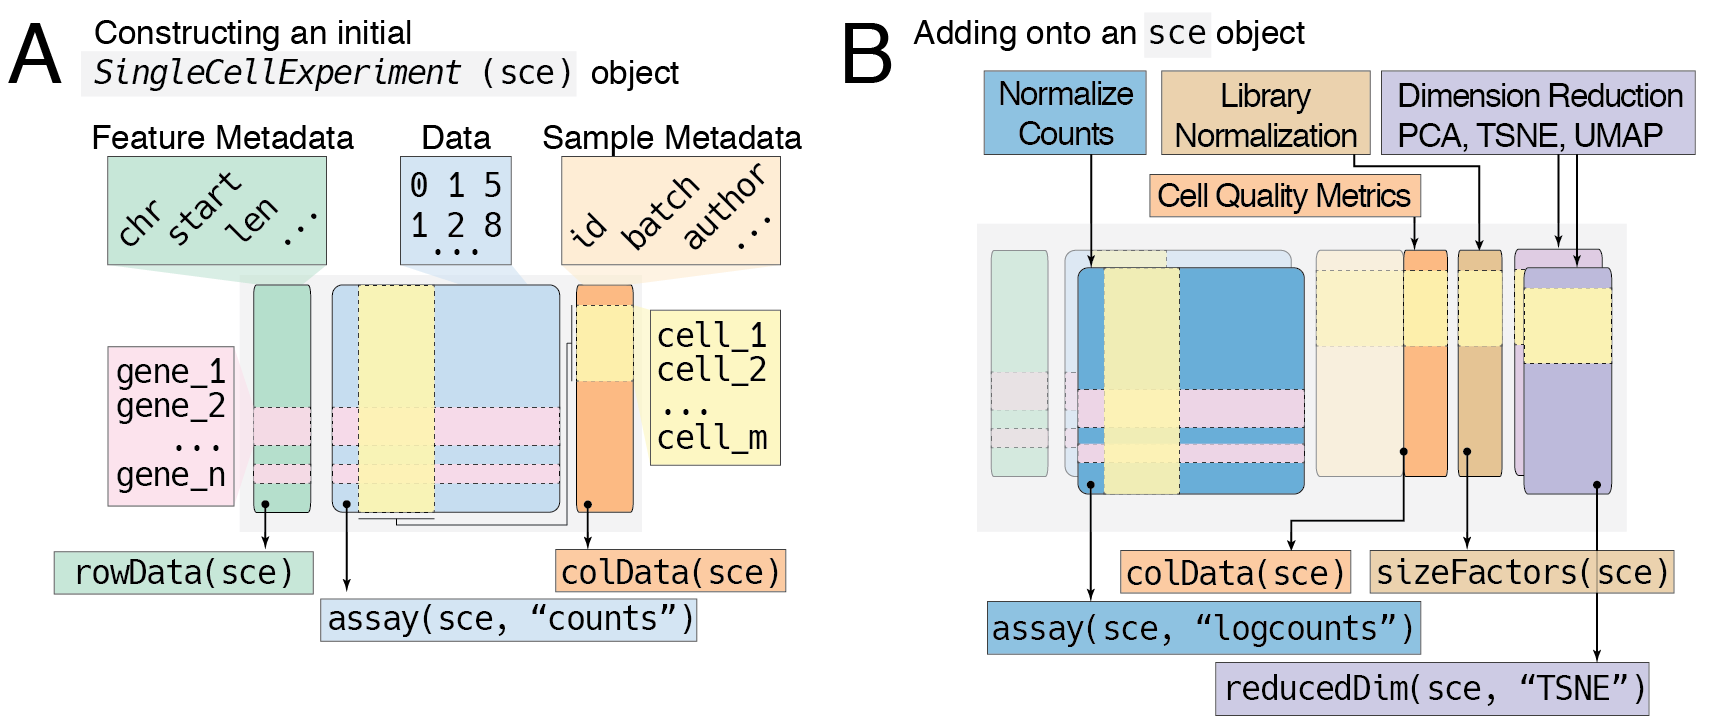
\includegraphics{_img/singlecellexperiment.png}
\caption{Figure 1. Overview of the SingleCellExperiment object}
\end{figure}

\hypertarget{primary-data-the-assays-slot}{%
\subsection{\texorpdfstring{Primary Data: The \texttt{assays} Slot}{Primary Data: The assays Slot}}\label{primary-data-the-assays-slot}}

The \texttt{SingleCellExperiment} (\texttt{sce}) object is the basis of single-cell analytical applications based in Bioconductor. The \texttt{sce} object is an \href{https://adv-r.hadley.nz/s4.html}{S4 object}, which in essence provides a more formalized approach towards construction and accession of data compared to other methods available in R. The utility of S4 comes from validity checks that ensure that safe data manipulation, and most important for our discussion, from its extensibility through \emph{slots}.

If we imagine the \texttt{sce} object to be a ship, the \emph{slots} of \texttt{sce} can be thought of as individual cargo boxes - each exists as a separate entity \emph{within} the \texttt{sce} object. Furthermore, each slot contains data that arrives in its own format. To extend the metaphor, we can imagine that different variations of cargo boxes are required for fruits versus bricks. In the case of \texttt{sce}, certain slots expect numeric matrices, whereas others may expect data frames.

To construct a rudimentary \texttt{sce} object, all we need is a single slot:

\begin{itemize}
\tightlist
\item
  \texttt{assays} slot: contains primary data such as counts in list, where each entry of the list is in a matrix format, where rows correspond to features (genes) and columns correspond to samples (cells) (\emph{Figure 1A, blue box})
\end{itemize}

Let's start simple by generating three cells worth of count data across ten genes.

\begin{Shaded}
\begin{Highlighting}[]
\NormalTok{counts_matrix <-}\StringTok{ }\KeywordTok{data.frame}\NormalTok{(}\DataTypeTok{cell_1 =} \KeywordTok{rpois}\NormalTok{(}\DecValTok{10}\NormalTok{, }\DecValTok{10}\NormalTok{), }
                    \DataTypeTok{cell_2 =} \KeywordTok{rpois}\NormalTok{(}\DecValTok{10}\NormalTok{, }\DecValTok{10}\NormalTok{), }
                    \DataTypeTok{cell_3 =} \KeywordTok{rpois}\NormalTok{(}\DecValTok{10}\NormalTok{, }\DecValTok{30}\NormalTok{))}
\KeywordTok{rownames}\NormalTok{(counts_matrix) <-}\StringTok{ }\KeywordTok{paste0}\NormalTok{(}\StringTok{"gene_"}\NormalTok{, }\DecValTok{1}\OperatorTok{:}\DecValTok{10}\NormalTok{)}
\NormalTok{counts_matrix <-}\StringTok{ }\KeywordTok{as.matrix}\NormalTok{(counts_matrix) }\CommentTok{# must be a matrix object!}
\end{Highlighting}
\end{Shaded}

From this, we can now construct our first \texttt{SingleCellExperiment} object, using the defined \emph{constructor}, \texttt{SingleCellExperiment()}. Note that we provide our data as a \emph{named} \emph{list}, and each entry of the list is a \emph{matrix}. Here, we name the \texttt{counts\_matrix} entry as simply \texttt{counts} within the list.

\begin{Shaded}
\begin{Highlighting}[]
\NormalTok{sce <-}\StringTok{ }\KeywordTok{SingleCellExperiment}\NormalTok{(}\DataTypeTok{assays =} \KeywordTok{list}\NormalTok{(}\DataTypeTok{counts =}\NormalTok{ counts_matrix))}
\end{Highlighting}
\end{Shaded}

To inspect the object, we can simply type \texttt{sce} into the console to see some pertinent information, which will display an overview of the various slots available to us (which may or may not have any data).

\begin{Shaded}
\begin{Highlighting}[]
\NormalTok{sce}
\end{Highlighting}
\end{Shaded}

\begin{verbatim}
## class: SingleCellExperiment 
## dim: 10 3 
## metadata(0):
## assays(1): counts
## rownames(10): gene_1 gene_2 ... gene_9 gene_10
## rowData names(0):
## colnames(3): cell_1 cell_2 cell_3
## colData names(0):
## reducedDimNames(0):
## spikeNames(0):
\end{verbatim}

To access the count data we just supplied, we can do any one of the following:

\begin{itemize}
\tightlist
\item
  \texttt{assay(sce,\ "counts")} - this is the most general method, where we can supply the name of the assay as the second argument.
\item
  \texttt{counts(sce)} - this is the same as the above, but \emph{only} works for assays with the special name \texttt{"counts"}.
\end{itemize}

\begin{Shaded}
\begin{Highlighting}[]
\KeywordTok{counts}\NormalTok{(sce)}
\end{Highlighting}
\end{Shaded}

\begin{verbatim}
##         cell_1 cell_2 cell_3
## gene_1      14     11     28
## gene_2       6      9     27
## gene_3       8      8     23
## gene_4       7      8     27
## gene_5      10      8     40
## gene_6      11     11     35
## gene_7       5     11     18
## gene_8      14      9     24
## gene_9      16      9     27
## gene_10      8     13     30
\end{verbatim}

\begin{Shaded}
\begin{Highlighting}[]
\CommentTok{## assay(sce, "counts") ## same as above in this special case}
\end{Highlighting}
\end{Shaded}

\hypertarget{extending-the-assays-slot}{%
\subsection{\texorpdfstring{Extending the \texttt{assays} Slot}{Extending the assays Slot}}\label{extending-the-assays-slot}}

What makes the \texttt{assay} slot especially powerful is that it can hold \emph{multiple} representations of the primary data. This is especially useful for storing a \emph{normalized} version of the data. We can do just that as shown below, using the \texttt{scran} and \texttt{scater} packages to compute a log-count normalized representation of the initial primary data.

Note that here, we overwrite our previous \texttt{sce} upon reassigning the results to \texttt{sce} - this is because these functions \emph{return} a \texttt{SingleCellExperiment} object. Some functions - especially those outside of single-cell oriented Bioconductor packages - do not, in which case you will need to append your results to the \texttt{sce} object (see below).

\begin{Shaded}
\begin{Highlighting}[]
\NormalTok{sce <-}\StringTok{ }\NormalTok{scran}\OperatorTok{::}\KeywordTok{computeSumFactors}\NormalTok{(sce)}
\NormalTok{sce <-}\StringTok{ }\NormalTok{scater}\OperatorTok{::}\KeywordTok{normalize}\NormalTok{(sce)}
\end{Highlighting}
\end{Shaded}

Viewing the object again, we see that these functions added some new entries:

\begin{Shaded}
\begin{Highlighting}[]
\NormalTok{sce}
\end{Highlighting}
\end{Shaded}

\begin{verbatim}
## class: SingleCellExperiment 
## dim: 10 3 
## metadata(1): log.exprs.offset
## assays(2): counts logcounts
## rownames(10): gene_1 gene_2 ... gene_9 gene_10
## rowData names(0):
## colnames(3): cell_1 cell_2 cell_3
## colData names(0):
## reducedDimNames(0):
## spikeNames(0):
\end{verbatim}

Specifically, we see that the \texttt{assays} slot has grown to be comprised of two entries: \texttt{counts} (our initial data) and \texttt{logcounts} (the normalized data). Similar to \texttt{counts}, the \texttt{logcounts} name is a special name which lets us access it simply by typing \texttt{logcounts(sce)}, although the longhand version works just as well.

\begin{Shaded}
\begin{Highlighting}[]
\KeywordTok{logcounts}\NormalTok{(sce)}
\end{Highlighting}
\end{Shaded}

\begin{verbatim}
##         cell_1 cell_2 cell_3
## gene_1    4.55   4.24   4.08
## gene_2    3.41   3.97   4.03
## gene_3    3.79   3.81   3.81
## gene_4    3.61   3.81   4.03
## gene_5    4.09   3.81   4.57
## gene_6    4.22   4.24   4.38
## gene_7    3.17   4.24   3.49
## gene_8    4.55   3.97   3.87
## gene_9    4.73   3.97   4.03
## gene_10   3.79   4.47   4.17
\end{verbatim}

\begin{Shaded}
\begin{Highlighting}[]
\CommentTok{## assay(sce, "logcounts") ## same as above}
\end{Highlighting}
\end{Shaded}

Notice that the data before had a severe discrepancy in counts between cells 1/2 versus 3, and that normalization has ameliorated this difference.

To look at all the available assays within \texttt{sce}, we can type:

\begin{Shaded}
\begin{Highlighting}[]
\KeywordTok{assays}\NormalTok{(sce)}
\end{Highlighting}
\end{Shaded}

\begin{verbatim}
## List of length 2
## names(2): counts logcounts
\end{verbatim}

While the functions above demonstrate automatic addition of assays to our \texttt{sce} object, there may be cases where we want to perform our own calculations and save the result into the \texttt{assays} slot. In particular, this is important for using functions that do \emph{not} return your \texttt{SingleCellExperiment} object.

Let's append a new version of the data that has been offset by \texttt{+100}.

\begin{Shaded}
\begin{Highlighting}[]
\NormalTok{counts_}\DecValTok{100}\NormalTok{ <-}\StringTok{ }\KeywordTok{assay}\NormalTok{(sce, }\StringTok{"counts"}\NormalTok{) }\OperatorTok{+}\StringTok{ }\DecValTok{100}
\KeywordTok{assay}\NormalTok{(sce, }\StringTok{"counts_100"}\NormalTok{) <-}\StringTok{ }\NormalTok{counts_}\DecValTok{100} \CommentTok{# assign a new entry to assays slot}
\end{Highlighting}
\end{Shaded}

Then we can use the accessor \texttt{assays()} (notice this is plural!) to see all our entries into the \texttt{assay} slot that we have made so far. Note that to see the \emph{names} of all the assays, we use the plural \texttt{assays()} accessor, and to retrieve a single assay entry (as a matrix) we use the singular \texttt{assay()} accessor, providing the name of the assay we wish to retrieve as above.

\begin{Shaded}
\begin{Highlighting}[]
\KeywordTok{assays}\NormalTok{(sce)}
\end{Highlighting}
\end{Shaded}

\begin{verbatim}
## List of length 3
## names(3): counts logcounts counts_100
\end{verbatim}

These entries are also seen on the default view of \texttt{sce}:

\begin{Shaded}
\begin{Highlighting}[]
\NormalTok{sce}
\end{Highlighting}
\end{Shaded}

\begin{verbatim}
## class: SingleCellExperiment 
## dim: 10 3 
## metadata(1): log.exprs.offset
## assays(3): counts logcounts counts_100
## rownames(10): gene_1 gene_2 ... gene_9 gene_10
## rowData names(0):
## colnames(3): cell_1 cell_2 cell_3
## colData names(0):
## reducedDimNames(0):
## spikeNames(0):
\end{verbatim}

This sort of extension of the \texttt{assays} slot is represented graphically in \emph{Figure 1B (dark blue box)}, showing the addition of the \texttt{logcounts} matrix into the \texttt{assays} slot.

In a similar manner, many of the slots of \texttt{sce} are extendable through assignment as shown above, thus allowing for myriad custom functionality as needed for interoperability with functions outside of single-cell oriented Bioconductor packages.

\hypertarget{column-metadata-coldata-slot}{%
\subsection{\texorpdfstring{Column (Meta)Data: \texttt{colData} Slot}{Column (Meta)Data: colData Slot}}\label{column-metadata-coldata-slot}}

To further annotate our \texttt{sce} object, one of the first and most useful pieces of information is adding on metadata that describes the columns of our primary data, e.g.~describing the samples or cells of our experiment. This data is entered into the \texttt{colData} slot:

\begin{itemize}
\tightlist
\item
  \texttt{colData} slot: metadata that describes that samples (cells) provided as a \texttt{data.frame} or (\texttt{DataFrame} if appending), where rows correspond to cells, and columns correspond to the sample (cells) metadata features (e.g.~id, batch, author, etc.) (\emph{Figure 1A, orange box}).
\end{itemize}

So, let's come up with some metadata for the cells, starting with a batch variable, where cells 1 and 2 are in batch 1, and cell 3 is from batch 2.

\begin{Shaded}
\begin{Highlighting}[]
\NormalTok{cell_metadata <-}\StringTok{ }\KeywordTok{data.frame}\NormalTok{(}\DataTypeTok{batch =} \KeywordTok{c}\NormalTok{(}\DecValTok{1}\NormalTok{, }\DecValTok{1}\NormalTok{, }\DecValTok{2}\NormalTok{))}
\KeywordTok{rownames}\NormalTok{(cell_metadata) <-}\StringTok{ }\KeywordTok{paste0}\NormalTok{(}\StringTok{"cell_"}\NormalTok{, }\DecValTok{1}\OperatorTok{:}\DecValTok{3}\NormalTok{)}
\end{Highlighting}
\end{Shaded}

Now, we can take two approaches - either append the \texttt{cell\_metadata} to our existing \texttt{sce}, or start from scratch via the \texttt{SingleCellExperiment()} constructor and provide it from the get go. We'll start from scratch for now, but will also show how to append the data as well:

\begin{Shaded}
\begin{Highlighting}[]
\CommentTok{## From scratch:}
\NormalTok{sce <-}\StringTok{ }\KeywordTok{SingleCellExperiment}\NormalTok{(}\DataTypeTok{assays =} \KeywordTok{list}\NormalTok{(}\DataTypeTok{counts =}\NormalTok{ counts_matrix),}
                           \DataTypeTok{colData =}\NormalTok{ cell_metadata)}

\CommentTok{## Appending to existing object (requires DataFrame() coercion)}
\CommentTok{## colData(sce) <- DataFrame(cell_metadata)}
\end{Highlighting}
\end{Shaded}

Similar to \texttt{assays}, we can see our colData is now populated from the default view of \texttt{sce}:

\begin{Shaded}
\begin{Highlighting}[]
\NormalTok{sce}
\end{Highlighting}
\end{Shaded}

\begin{verbatim}
## class: SingleCellExperiment 
## dim: 10 3 
## metadata(0):
## assays(1): counts
## rownames(10): gene_1 gene_2 ... gene_9 gene_10
## rowData names(0):
## colnames(3): cell_1 cell_2 cell_3
## colData names(1): batch
## reducedDimNames(0):
## spikeNames(0):
\end{verbatim}

And furthermore access our column (meta)data with the accessor, \texttt{colData()}:

\begin{Shaded}
\begin{Highlighting}[]
\KeywordTok{colData}\NormalTok{(sce)}
\end{Highlighting}
\end{Shaded}

\begin{verbatim}
## DataFrame with 3 rows and 1 column
##            batch
##        <numeric>
## cell_1         1
## cell_2         1
## cell_3         2
\end{verbatim}

Finally, some packages automatically add to the \texttt{colData} slot, for example, the \texttt{scater} package features a function, \texttt{calculateQCMetrics()}, which appends a lot of quality control data. Here we show the first five columns of \texttt{colData(sce)} with the quality control metrics appended to it.

\begin{Shaded}
\begin{Highlighting}[]
\NormalTok{sce <-}\StringTok{ }\NormalTok{scater}\OperatorTok{::}\KeywordTok{calculateQCMetrics}\NormalTok{(sce)}
\KeywordTok{colData}\NormalTok{(sce)[, }\DecValTok{1}\OperatorTok{:}\DecValTok{5}\NormalTok{]}
\end{Highlighting}
\end{Shaded}

\begin{verbatim}
## DataFrame with 3 rows and 5 columns
##            batch is_cell_control total_features_by_counts
##        <numeric>       <logical>                <integer>
## cell_1         1           FALSE                       10
## cell_2         1           FALSE                       10
## cell_3         2           FALSE                       10
##        log10_total_features_by_counts total_counts
##                             <numeric>    <integer>
## cell_1               1.04139268515823           99
## cell_2               1.04139268515823           97
## cell_3               1.04139268515823          279
\end{verbatim}

\hypertarget{using-coldata-for-subsetting}{%
\subsubsection{\texorpdfstring{Using \texttt{colData} for Subsetting}{Using colData for Subsetting}}\label{using-coldata-for-subsetting}}

A common operation with \texttt{colData} is its use in subsetting. One simple way to access \texttt{colData} is through the use of the \texttt{\$} operator, which is a shortcut for accessing a variable within the \texttt{colData} slot:

\begin{Shaded}
\begin{Highlighting}[]
\NormalTok{sce}\OperatorTok{$}\NormalTok{batch}
\end{Highlighting}
\end{Shaded}

\begin{verbatim}
## [1] 1 1 2
\end{verbatim}

\begin{Shaded}
\begin{Highlighting}[]
\CommentTok{## colData(sce)$batch # same as above}
\end{Highlighting}
\end{Shaded}

If we only wanted cells within batch 1, we could subset our sce object as follows (remember, we subset on the \emph{columns} in this case because we are filtering by cells/samples here).

\begin{Shaded}
\begin{Highlighting}[]
\NormalTok{sce[, sce}\OperatorTok{$}\NormalTok{batch }\OperatorTok{==}\StringTok{ }\DecValTok{1}\NormalTok{]}
\end{Highlighting}
\end{Shaded}

\begin{verbatim}
## class: SingleCellExperiment 
## dim: 10 2 
## metadata(0):
## assays(1): counts
## rownames(10): gene_1 gene_2 ... gene_9 gene_10
## rowData names(7): is_feature_control mean_counts ... total_counts
##   log10_total_counts
## colnames(2): cell_1 cell_2
## colData names(10): batch is_cell_control ...
##   pct_counts_in_top_200_features pct_counts_in_top_500_features
## reducedDimNames(0):
## spikeNames(0):
\end{verbatim}

\hypertarget{feature-metadata-rowdatarowranges}{%
\subsection{\texorpdfstring{Feature Metadata: \texttt{rowData}/\texttt{rowRanges}}{Feature Metadata: rowData/rowRanges}}\label{feature-metadata-rowdatarowranges}}

Lastly, the rows also have their own metadata slot to store information that pertains to the features of the \texttt{sce} object:

\begin{itemize}
\tightlist
\item
  \texttt{rowData} slot: contains data in a \texttt{data.frame} (\texttt{DataFrame}) format that describes aspects of the data corresponding to the rows of the primary data (\emph{Figure 1A, green box}).
\end{itemize}

Furthermore, there is a special slot which pertains to features with genomic coordinates:

\begin{itemize}
\tightlist
\item
  \texttt{rowRanges} slot: contains data in a \texttt{GRangesList} (where each entry is a \texttt{GenomicRanges} format) that describes the chromosome, start, and end coordinates of the features (genes, genomic regions).
\end{itemize}

Both of these can be accessed via their respective accessors, \texttt{rowRanges()} and \texttt{rowData()}. In our case, \texttt{rowRanges(sce)} produces an empty list:

\begin{Shaded}
\begin{Highlighting}[]
\KeywordTok{rowRanges}\NormalTok{(sce) }\CommentTok{# empty}
\end{Highlighting}
\end{Shaded}

\begin{verbatim}
## GRangesList object of length 10:
## $gene_1 
## GRanges object with 0 ranges and 0 metadata columns:
##    seqnames    ranges strand
##       <Rle> <IRanges>  <Rle>
## 
## $gene_2 
## GRanges object with 0 ranges and 0 metadata columns:
##      seqnames ranges strand
## 
## $gene_3 
## GRanges object with 0 ranges and 0 metadata columns:
##      seqnames ranges strand
## 
## ...
## <7 more elements>
## -------
## seqinfo: no sequences
\end{verbatim}

However, our call to \texttt{calculateQCMetrics(sce)} in the prior section filled in the \texttt{rowData} slot of our \texttt{sce} object, as we can see below (only the first three columns are shown for brevity):

\begin{Shaded}
\begin{Highlighting}[]
\KeywordTok{rowData}\NormalTok{(sce)[, }\DecValTok{1}\OperatorTok{:}\DecValTok{3}\NormalTok{]}
\end{Highlighting}
\end{Shaded}

\begin{verbatim}
## DataFrame with 10 rows and 3 columns
##         is_feature_control      mean_counts log10_mean_counts
##                  <logical>        <numeric>         <numeric>
## gene_1               FALSE 17.6666666666667  1.27106677228654
## gene_2               FALSE               14  1.17609125905568
## gene_3               FALSE               13  1.14612803567824
## gene_4               FALSE               14  1.17609125905568
## gene_5               FALSE 19.3333333333333   1.3082085802911
## gene_6               FALSE               19  1.30102999566398
## gene_7               FALSE 11.3333333333333  1.09108046934733
## gene_8               FALSE 15.6666666666667  1.22184874961636
## gene_9               FALSE 17.3333333333333  1.26324143477458
## gene_10              FALSE               17  1.25527250510331
\end{verbatim}

In a similar fashion to the \texttt{colData} slot, such feature metadata could be provided at the onset when creating the \texttt{SingleCellExperiment} object, which we leave up to the reader as an exercise.

\hypertarget{subsetting-with-on-rows}{%
\subsubsection{Subsetting with on Rows}\label{subsetting-with-on-rows}}

To subset an \texttt{sce} object down at the feature/gene level, we can do a row subsetting operation similar to other R objects, by supplying either numeric indices or a vector of names:

\begin{Shaded}
\begin{Highlighting}[]
\NormalTok{sce[}\KeywordTok{c}\NormalTok{(}\StringTok{"gene_1"}\NormalTok{, }\StringTok{"gene_4"}\NormalTok{), ]}
\end{Highlighting}
\end{Shaded}

\begin{verbatim}
## class: SingleCellExperiment 
## dim: 2 3 
## metadata(0):
## assays(1): counts
## rownames(2): gene_1 gene_4
## rowData names(7): is_feature_control mean_counts ... total_counts
##   log10_total_counts
## colnames(3): cell_1 cell_2 cell_3
## colData names(10): batch is_cell_control ...
##   pct_counts_in_top_200_features pct_counts_in_top_500_features
## reducedDimNames(0):
## spikeNames(0):
\end{verbatim}

\begin{Shaded}
\begin{Highlighting}[]
\CommentTok{## sce[c(1, 4), ] # same as above in this case}
\end{Highlighting}
\end{Shaded}

\hypertarget{size-factors-slot-sizefactors}{%
\subsection{\texorpdfstring{Size Factors Slot: \texttt{sizeFactors}}{Size Factors Slot: sizeFactors}}\label{size-factors-slot-sizefactors}}

Briefly, we already encountered this via the \texttt{scran::computeSumFactors(sce)} call, which adds a \texttt{sizeFactors} slot:

\begin{itemize}
\tightlist
\item
  \texttt{sizeFactors} slot: contains information in a numeric vector regarding the sample/cell normalization factors used to produce a normalize data representation (\emph{Figure 1B, brown box})
\end{itemize}

\begin{Shaded}
\begin{Highlighting}[]
\NormalTok{sce <-}\StringTok{ }\NormalTok{scran}\OperatorTok{::}\KeywordTok{computeSumFactors}\NormalTok{(sce)}
\NormalTok{sce <-}\StringTok{ }\NormalTok{scater}\OperatorTok{::}\KeywordTok{normalize}\NormalTok{(sce)}
\KeywordTok{sizeFactors}\NormalTok{(sce)}
\end{Highlighting}
\end{Shaded}

\begin{verbatim}
## [1] 0.625 0.613 1.762
\end{verbatim}

\hypertarget{a-brief-recap-from-se-to-sce}{%
\section{\texorpdfstring{A Brief Recap: From \texttt{se} to \texttt{sce}}{A Brief Recap: From se to sce}}\label{a-brief-recap-from-se-to-sce}}

So far, we have covered the \texttt{assays} (primary data), \texttt{colData} (sample metadata), \texttt{rowData}/\texttt{rowRanges} (feature metadata), and \texttt{sizeFactors} slots of \texttt{SingleCellExperiment}.

What is important to note is that the \texttt{SingleCellExperiment} class \emph{derives} from the \texttt{SummarizedExperiment} (\texttt{se}) class, its predecessor, and in particular inherits the aforementioned slots. As such, much of the \texttt{SummarizedExperiment} functionality is retained in \texttt{SingleCellExperiment}. This allows existing methods that work with \texttt{SummarizedExperiment} to work similarly on \texttt{SingleCellExperiment} objects.

So what's new about the \texttt{SingleCellExperiment} class then? For our discussion, the most important change is the addition of a new slot called \texttt{reducedDims}.

\hypertarget{the-reduceddims-slot}{%
\section{\texorpdfstring{The \texttt{reducedDims} Slot}{The reducedDims Slot}}\label{the-reduceddims-slot}}

The \texttt{reducedDims} slot is a new addition which is specially designed to store the reduced dimensionality representations of primary data, such as PCA, tSNE, UMAP, and others.

\begin{itemize}
\tightlist
\item
  \texttt{reducedDims} slot: contains a list of numeric \texttt{matrix} entries which describe dimensionality reduced representations of the primary data, such that rows represent the columns of the primary data (aka the samples/cells), and columns represent the dimensions
\end{itemize}

Most importantly, just like the \texttt{assays} slot, the \texttt{reducedDims} slot can hold a list of many entries. So, it can hold a PCA, TSNE, and UMAP representation of a given dataset all within the \texttt{reducedDims} slot.

In our example, we can calculate a PCA representation of our data as follows using the \texttt{scater} package function \texttt{runPCA()}. We see that the \texttt{sce} now shows a new \texttt{reducedDim} and that the accessor \texttt{reducedDim()} produces the results of running PCA on the normalized data from \texttt{logcounts(sce)}.

\begin{Shaded}
\begin{Highlighting}[]
\NormalTok{sce <-}\StringTok{ }\NormalTok{scater}\OperatorTok{::}\KeywordTok{runPCA}\NormalTok{(sce)}
\KeywordTok{reducedDim}\NormalTok{(sce, }\StringTok{"PCA"}\NormalTok{)}
\end{Highlighting}
\end{Shaded}

\begin{verbatim}
##          PC1   PC2
## cell_1 -3.12  0.25
## cell_2  1.19 -1.71
## cell_3  1.93  1.46
## attr(,"percentVar")
## [1] 0.743 0.257
\end{verbatim}

From this, we can also calculate a tSNE representation using the \texttt{scater} package function \texttt{runTSNE()}, and see that it can be seen both in the default view of \texttt{sce} and via accession:

\begin{Shaded}
\begin{Highlighting}[]
\NormalTok{sce <-}\StringTok{ }\NormalTok{scater}\OperatorTok{::}\KeywordTok{runTSNE}\NormalTok{(sce, }\DataTypeTok{perplexity =} \FloatTok{0.1}\NormalTok{)}
\end{Highlighting}
\end{Shaded}

\begin{verbatim}
## Perplexity should be lower than K!
\end{verbatim}

\begin{Shaded}
\begin{Highlighting}[]
\KeywordTok{reducedDim}\NormalTok{(sce, }\StringTok{"TSNE"}\NormalTok{)}
\end{Highlighting}
\end{Shaded}

\begin{verbatim}
##         [,1]  [,2]
## cell_1  3012  4852
## cell_2  2686 -4990
## cell_3 -5697   138
\end{verbatim}

We can view the names of all our entries in the \texttt{reducedDims} slot via the accessor, \texttt{reducedDims()} (notice that this is plural, and thus not the same as \texttt{reducedDim()}:

\begin{Shaded}
\begin{Highlighting}[]
\KeywordTok{reducedDims}\NormalTok{(sce)}
\end{Highlighting}
\end{Shaded}

\begin{verbatim}
## List of length 2
## names(2): PCA TSNE
\end{verbatim}

Now, say we have a different dimensionality reduction approach which has not yet been implemented with \texttt{SingleCellExperiment} objects in mind. For example, let's say we want to try the \texttt{umap()} function as implemented in the \texttt{uwot} package (which is a much faster version of the default \texttt{umap} implementation currently in \texttt{scater}).

Similar to how we extended the \texttt{assays} slot with our own custom entry of \texttt{counts\_100}, we can do similarly for the \texttt{reducedDims} slot:

\begin{Shaded}
\begin{Highlighting}[]
\NormalTok{u <-}\StringTok{ }\NormalTok{uwot}\OperatorTok{::}\KeywordTok{umap}\NormalTok{(}\KeywordTok{t}\NormalTok{(}\KeywordTok{logcounts}\NormalTok{(sce)), }\DataTypeTok{n_neighbors =} \DecValTok{2}\NormalTok{)}
\KeywordTok{reducedDim}\NormalTok{(sce, }\StringTok{"UMAP_uwot"}\NormalTok{) <-}\StringTok{ }\NormalTok{u}

\KeywordTok{reducedDim}\NormalTok{(sce, }\StringTok{"UMAP_uwot"}\NormalTok{)}
\end{Highlighting}
\end{Shaded}

\begin{verbatim}
##          [,1]   [,2]
## cell_1 -0.650 -0.321
## cell_2  0.373  0.523
## cell_3  0.277 -0.202
## attr(,"scaled:center")
## [1]  1.76 -9.74
\end{verbatim}

And we can also see its entry when we look at the \texttt{reducedDims()} accessor output:

\begin{Shaded}
\begin{Highlighting}[]
\KeywordTok{reducedDims}\NormalTok{(sce)}
\end{Highlighting}
\end{Shaded}

\begin{verbatim}
## List of length 3
## names(3): PCA TSNE UMAP_uwot
\end{verbatim}

\hypertarget{one-more-thing-metadata-slot}{%
\section{\texorpdfstring{One More Thing: \texttt{metadata} Slot}{One More Thing: metadata Slot}}\label{one-more-thing-metadata-slot}}

Some analyses produce results that do not fit into the aforementioned slots. Thankfully, there is a slot just for this type of messy data, and in fact, can accommodate any type of data, so long as it is in a named list:

\begin{itemize}
\tightlist
\item
  \texttt{metadata} slot: a named list of entries, where each entry in the list can be anything you want it to be
\end{itemize}

For example, say we have some favorite genes, such as highly variable genes, we want to save inside of \texttt{sce} for use in our analysis at a later point. We can do this simply by appending to the metadata slot as follows:

\begin{Shaded}
\begin{Highlighting}[]
\NormalTok{my_genes <-}\StringTok{ }\KeywordTok{c}\NormalTok{(}\StringTok{"gene_1"}\NormalTok{, }\StringTok{"gene_5"}\NormalTok{)}
\KeywordTok{metadata}\NormalTok{(sce) <-}\StringTok{ }\KeywordTok{list}\NormalTok{(}\DataTypeTok{favorite_genes =}\NormalTok{ my_genes)}
\KeywordTok{metadata}\NormalTok{(sce)}
\end{Highlighting}
\end{Shaded}

\begin{verbatim}
## $favorite_genes
## [1] "gene_1" "gene_5"
\end{verbatim}

Similarly, we can append more information via the \texttt{\$} operator:

\begin{Shaded}
\begin{Highlighting}[]
\NormalTok{your_genes <-}\StringTok{ }\KeywordTok{c}\NormalTok{(}\StringTok{"gene_4"}\NormalTok{, }\StringTok{"gene_8"}\NormalTok{)}
\KeywordTok{metadata}\NormalTok{(sce)}\OperatorTok{$}\NormalTok{your_genes <-}\StringTok{ }\NormalTok{your_genes}
\KeywordTok{metadata}\NormalTok{(sce)}
\end{Highlighting}
\end{Shaded}

\begin{verbatim}
## $favorite_genes
## [1] "gene_1" "gene_5"
## 
## $your_genes
## [1] "gene_4" "gene_8"
\end{verbatim}

\hypertarget{about-spike-ins}{%
\section{About Spike-Ins}\label{about-spike-ins}}

You might have noticed that the \texttt{sce} default view produces an entry with \texttt{spikeNames}. The \texttt{SingleCellExperiment} object contains some special considerations for experiments with spike-in (ERCC) controls. We leave this to the interested reader to learn more about in the \href{https://bioconductor.org/packages/release/bioc/vignettes/SingleCellExperiment/inst/doc/intro.html}{\texttt{SingleCellExperiment} introductory vignette}.

\hypertarget{working-with-singlecellexperiment}{%
\section{\texorpdfstring{Working with \emph{SingleCellExperiment}}{Working with SingleCellExperiment}}\label{working-with-singlecellexperiment}}

\emph{Figure 1C} shows an example workflow that uses the \texttt{SingleCellExperiment} object as its base, and similar to our walkthrough of the \texttt{sce} class above, continually appends new entries to save the results of the analysis. In the workflows that follow in this book, we will be similarly appending to an initial \texttt{sce} object many of our analytical results.

\hypertarget{part-workflows}{%
\part{Workflows}\label{part-workflows}}

\hypertarget{about-the-data}{%
\chapter{About the Data}\label{about-the-data}}

\hypertarget{x-genomics-pbmc-data}{%
\section{10X Genomics PBMC Data}\label{x-genomics-pbmc-data}}

Bioconductor versions, PBMC4k/PBMC3k.

\hypertarget{human-cell-atlas}{%
\section{Human Cell Atlas}\label{human-cell-atlas}}

Bioconductor access.

\begin{Shaded}
\begin{Highlighting}[]
\NormalTok{d =}\StringTok{ }\KeywordTok{c}\NormalTok{(}\StringTok{'a'}\NormalTok{, }\StringTok{'b'}\NormalTok{)}
\end{Highlighting}
\end{Shaded}

\hypertarget{workflow-integrating-datasets}{%
\chapter{Workflow: Integrating Datasets}\label{workflow-integrating-datasets}}

The purpose of this case study is to demonstrate how to integrate multiple scRNA-seq datasets using R/Bioconductor packages. In this workflow, we go from preprocessing the data to integrating the data and visualizing it in a reduced dimensionality space to showcase the success of the integration approach using mutual nearest neighbors relative to a naive approach. This approach is helpful for ameliorating batch effects that can be introduced when combining data from different sequencing runs and/or platforms.

Here, we will be combining two datasets from 10X Genomics PBMC Data. One dataset is comprised of 3000 PBMCs from a healthy donor, and the other dataset is comprised of 4000 PBMCs from a different healthy donor. Our goal is to produce an integrated representation of this data to facilitate downstream analysis, such as clustering.

\hypertarget{package-requirements}{%
\section{Package Requirements}\label{package-requirements}}

These packages will be required for working through the vignette, and can be installed by running the code below. The data that we will be using comes from the \texttt{TENxPBMCData} package.

\begin{Shaded}
\begin{Highlighting}[]
\CommentTok{## required}
\NormalTok{BiocManager}\OperatorTok{::}\KeywordTok{install}\NormalTok{(}\KeywordTok{c}\NormalTok{(}\StringTok{'scater'}\NormalTok{, }\StringTok{'scran'}\NormalTok{, }\StringTok{'limma'}\NormalTok{, }\StringTok{'TENxPBMCData'}\NormalTok{))}

\CommentTok{## suggested}
\NormalTok{BiocManager}\OperatorTok{::}\KeywordTok{install}\NormalTok{(}\KeywordTok{c}\NormalTok{(}\StringTok{'BiocParallel'}\NormalTok{, }\StringTok{'BiocNeighbors'}\NormalTok{))}
\end{Highlighting}
\end{Shaded}

\begin{Shaded}
\begin{Highlighting}[]
\KeywordTok{library}\NormalTok{(scater)}
\KeywordTok{library}\NormalTok{(scran)}
\KeywordTok{library}\NormalTok{(limma)}
\KeywordTok{library}\NormalTok{(TENxPBMCData)}
\KeywordTok{library}\NormalTok{(BiocParallel)}
\KeywordTok{library}\NormalTok{(BiocNeighbors)}
\end{Highlighting}
\end{Shaded}

\hypertarget{loading-the-data}{%
\section{Loading the Data}\label{loading-the-data}}

Here we will be combining two different runs of scRNA-seq data - each from different healthy donors, and comprised of either 3000 cells (\texttt{pbmc3k}) or 4000 cells (\texttt{pbmc4k}). Note that these objects are already \texttt{SingleCellExperiment} objects.

\begin{Shaded}
\begin{Highlighting}[]
\NormalTok{pbmc3k <-}\StringTok{ }\KeywordTok{TENxPBMCData}\NormalTok{(}\StringTok{'pbmc3k'}\NormalTok{)}
\NormalTok{pbmc4k <-}\StringTok{ }\KeywordTok{TENxPBMCData}\NormalTok{(}\StringTok{'pbmc4k'}\NormalTok{)}
\end{Highlighting}
\end{Shaded}

\hypertarget{preprocessing}{%
\section{Preprocessing}\label{preprocessing}}

Here we walk through the steps required to produce a clean expression matrix, taking the raw count data through to a normalized representation.

\hypertarget{working-with-common-genes}{%
\subsection{Working with Common Genes}\label{working-with-common-genes}}

First, we find intersection of gene names and keep only the entries that are in common between the two datasets. We then reduce each of the individual datasets down to these matching entries (\texttt{keep\_genes}) by subsetting.

\begin{Shaded}
\begin{Highlighting}[]
\NormalTok{keep_genes <-}\StringTok{ }\KeywordTok{intersect}\NormalTok{(}\KeywordTok{rownames}\NormalTok{(pbmc3k), }\KeywordTok{rownames}\NormalTok{(pbmc4k))}
\NormalTok{pbmc3k <-}\StringTok{ }\NormalTok{pbmc3k[}\KeywordTok{match}\NormalTok{(keep_genes, }\KeywordTok{rownames}\NormalTok{(pbmc3k)), ]}
\NormalTok{pbmc4k <-}\StringTok{ }\NormalTok{pbmc4k[}\KeywordTok{na.omit}\NormalTok{(}\KeywordTok{match}\NormalTok{(keep_genes, }\KeywordTok{rownames}\NormalTok{(pbmc4k))), ]}
\end{Highlighting}
\end{Shaded}

\hypertarget{cell-and-gene-quality-control}{%
\subsection{Cell and Gene Quality Control}\label{cell-and-gene-quality-control}}

First, for the combined data \texttt{sce} and the individual datasets \texttt{pbmc3k} and \texttt{pbmc4k}, we calculate essential quality control characteristics using the \texttt{scater} function \texttt{calculateQCMetrics()}. We then determine cells low quality cells by finding outliers with uncharacteristically low total counts or total number of features (genes) detected. We automate this into a function.

\begin{Shaded}
\begin{Highlighting}[]
\CommentTok{## For pbmc3k}
\NormalTok{pbmc3k <-}\StringTok{ }\KeywordTok{calculateQCMetrics}\NormalTok{(pbmc3k)}
\NormalTok{low_lib_pbmc3k <-}\StringTok{ }\KeywordTok{isOutlier}\NormalTok{(pbmc3k}\OperatorTok{$}\NormalTok{log10_total_counts, }\DataTypeTok{type=}\StringTok{"lower"}\NormalTok{, }\DataTypeTok{nmad=}\DecValTok{3}\NormalTok{)}
\NormalTok{low_genes_pbmc3k <-}\StringTok{ }\KeywordTok{isOutlier}\NormalTok{(pbmc3k}\OperatorTok{$}\NormalTok{log10_total_features_by_counts, }\DataTypeTok{type=}\StringTok{"lower"}\NormalTok{, }\DataTypeTok{nmad=}\DecValTok{3}\NormalTok{)}

\CommentTok{## For pbmc4k}
\NormalTok{pbmc4k <-}\StringTok{ }\KeywordTok{calculateQCMetrics}\NormalTok{(pbmc4k)}
\NormalTok{low_lib_pbmc4k <-}\StringTok{ }\KeywordTok{isOutlier}\NormalTok{(pbmc4k}\OperatorTok{$}\NormalTok{log10_total_counts, }\DataTypeTok{type=}\StringTok{"lower"}\NormalTok{, }\DataTypeTok{nmad=}\DecValTok{3}\NormalTok{)}
\NormalTok{low_genes_pbmc4k <-}\StringTok{ }\KeywordTok{isOutlier}\NormalTok{(pbmc4k}\OperatorTok{$}\NormalTok{log10_total_features_by_counts, }\DataTypeTok{type=}\StringTok{"lower"}\NormalTok{, }\DataTypeTok{nmad=}\DecValTok{3}\NormalTok{)}
\end{Highlighting}
\end{Shaded}

These results flag approximately 30 to 100 cells for removal from each of the datasets. We can then further subset our data to remove these cells by running the following:

\begin{Shaded}
\begin{Highlighting}[]
\NormalTok{pbmc3k <-}\StringTok{ }\NormalTok{pbmc3k[,}\OperatorTok{!}\NormalTok{(low_lib_pbmc3k }\OperatorTok{|}\StringTok{ }\NormalTok{low_genes_pbmc3k)]}
\NormalTok{pbmc4k <-}\StringTok{ }\NormalTok{pbmc4k[,}\OperatorTok{!}\NormalTok{(low_lib_pbmc4k }\OperatorTok{|}\StringTok{ }\NormalTok{low_genes_pbmc4k)]}
\end{Highlighting}
\end{Shaded}

\hypertarget{normalization}{%
\subsection{Normalization}\label{normalization}}

From here, we now compute the size factors using the \texttt{scran} package's \texttt{computeSumFactors()} function, and apply the size factors via the \texttt{scran} package's \texttt{normalize()} function to produce a new assay, \texttt{logcounts}, within each \texttt{SingleCellExperiment} object.

\begin{Shaded}
\begin{Highlighting}[]
\CommentTok{## compute the sizeFactors}
\NormalTok{pbmc3k <-}\StringTok{ }\KeywordTok{computeSumFactors}\NormalTok{(pbmc3k)}
\NormalTok{pbmc4k <-}\StringTok{ }\KeywordTok{computeSumFactors}\NormalTok{(pbmc4k)}

\CommentTok{## Normalize (using already calculated size factors)}
\NormalTok{pbmc3k <-}\StringTok{ }\KeywordTok{normalize}\NormalTok{(pbmc3k)}
\NormalTok{pbmc4k <-}\StringTok{ }\KeywordTok{normalize}\NormalTok{(pbmc4k)}
\end{Highlighting}
\end{Shaded}

\hypertarget{multibatch-normalization}{%
\subsection{Multibatch Normalization}\label{multibatch-normalization}}

We also rescale each batch to adjust for differences in sequencing depth between batches. The \texttt{multiBatchNorm()} function from the \texttt{scran} package recomputes log-normalized expression values after adjusting the size factors for systematic differences in coverage between \texttt{SingleCellExperiment} objects. The previously computed size factors only remove biases between cells within a single batch. This improves the quality of the correction step by removing one aspect of the technical differences between batches.

\begin{Shaded}
\begin{Highlighting}[]
\NormalTok{rescaled <-}\StringTok{ }\KeywordTok{multiBatchNorm}\NormalTok{(pbmc3k, pbmc4k)}
\NormalTok{pbmc3k <-}\StringTok{ }\NormalTok{rescaled[[}\DecValTok{1}\NormalTok{]]}
\NormalTok{pbmc4k <-}\StringTok{ }\NormalTok{rescaled[[}\DecValTok{2}\NormalTok{]]}
\end{Highlighting}
\end{Shaded}

\hypertarget{feature-selection}{%
\section{Feature Selection}\label{feature-selection}}

A key step across many data integration methods is the selection of informative features across the different experiments. This helps to speed up computation and possibly improve the resulting integration.

Once again, we rely on the \texttt{scran} package to identify the genes with the highest biological coefficient of variation, using the \texttt{trendVar()} and \texttt{decomposeVar()} functions to calculate the per gene variance and separate it into technical versus biological components. We perform this for each individual dataset:

\begin{Shaded}
\begin{Highlighting}[]
\NormalTok{fit_pbmc3k <-}\StringTok{ }\KeywordTok{trendVar}\NormalTok{(pbmc3k, }\DataTypeTok{use.spikes=}\OtherTok{FALSE}\NormalTok{) }
\NormalTok{dec_pbmc3k <-}\StringTok{ }\KeywordTok{decomposeVar}\NormalTok{(pbmc3k, fit_pbmc3k)}
\NormalTok{dec_pbmc3k}\OperatorTok{$}\NormalTok{Symbol_TENx <-}\StringTok{ }\KeywordTok{rowData}\NormalTok{(pbmc3k)}\OperatorTok{$}\NormalTok{Symbol_TENx}
\NormalTok{dec_pbmc3k <-}\StringTok{ }\NormalTok{dec_pbmc3k[}\KeywordTok{order}\NormalTok{(dec_pbmc3k}\OperatorTok{$}\NormalTok{bio, }\DataTypeTok{decreasing =} \OtherTok{TRUE}\NormalTok{), ]}

\NormalTok{fit_pbmc4k <-}\StringTok{ }\KeywordTok{trendVar}\NormalTok{(pbmc4k, }\DataTypeTok{use.spikes=}\OtherTok{FALSE}\NormalTok{) }
\NormalTok{dec_pbmc4k <-}\StringTok{ }\KeywordTok{decomposeVar}\NormalTok{(pbmc4k, fit_pbmc4k)}
\NormalTok{dec_pbmc4k}\OperatorTok{$}\NormalTok{Symbol_TENx <-}\StringTok{ }\KeywordTok{rowData}\NormalTok{(pbmc4k)}\OperatorTok{$}\NormalTok{Symbol_TENx}
\NormalTok{dec_pbmc4k <-}\StringTok{ }\NormalTok{dec_pbmc4k[}\KeywordTok{order}\NormalTok{(dec_pbmc4k}\OperatorTok{$}\NormalTok{bio, }\DataTypeTok{decreasing =} \OtherTok{TRUE}\NormalTok{), ]}
\end{Highlighting}
\end{Shaded}

Then select the most informative genes that are shared across \emph{both} datasets:

\begin{Shaded}
\begin{Highlighting}[]
\NormalTok{universe <-}\StringTok{ }\KeywordTok{intersect}\NormalTok{(}\KeywordTok{rownames}\NormalTok{(dec_pbmc3k), }\KeywordTok{rownames}\NormalTok{(dec_pbmc4k))}
\NormalTok{mean.bio <-}\StringTok{ }\NormalTok{(dec_pbmc3k[universe,}\StringTok{"bio"}\NormalTok{] }\OperatorTok{+}\StringTok{ }\NormalTok{dec_pbmc4k[universe,}\StringTok{"bio"}\NormalTok{])}\OperatorTok{/}\DecValTok{2}
\NormalTok{hvg_genes <-}\StringTok{ }\NormalTok{universe[mean.bio }\OperatorTok{>}\StringTok{ }\DecValTok{0}\NormalTok{]}
\end{Highlighting}
\end{Shaded}

\hypertarget{combining-the-datasets}{%
\section{Combining the Datasets}\label{combining-the-datasets}}

Finally, we combine the datasets into a unified \texttt{SingleCellExperiment} object for the downstream integration approaches, now that the data has been normalized (both within and between datasets) and the shared most informative features have been identified.

\begin{Shaded}
\begin{Highlighting}[]
\CommentTok{## total raw counts}
\NormalTok{counts_pbmc <-}\StringTok{ }\KeywordTok{cbind}\NormalTok{(}\KeywordTok{counts}\NormalTok{(pbmc3k), }\KeywordTok{counts}\NormalTok{(pbmc4k))}

\CommentTok{## total normalized counts (with multibatch normalization)}
\NormalTok{logcounts_pbmc <-}\StringTok{ }\KeywordTok{cbind}\NormalTok{(}\KeywordTok{logcounts}\NormalTok{(pbmc3k), }\KeywordTok{logcounts}\NormalTok{(pbmc4k))}

\NormalTok{sce <-}\StringTok{ }\KeywordTok{SingleCellExperiment}\NormalTok{( }
    \DataTypeTok{assays =} \KeywordTok{list}\NormalTok{(}\DataTypeTok{counts =}\NormalTok{ counts_pbmc, }\DataTypeTok{logcounts =}\NormalTok{ logcounts_pbmc),  }
    \DataTypeTok{rowData =} \KeywordTok{rowData}\NormalTok{(pbmc3k), }\CommentTok{# same as rowData(pbmc4k) }
    \DataTypeTok{colData =} \KeywordTok{rbind}\NormalTok{(}\KeywordTok{colData}\NormalTok{(pbmc3k), }\KeywordTok{colData}\NormalTok{(pbmc4k)) }
\NormalTok{) }
\end{Highlighting}
\end{Shaded}

For safekeeping, we will also store the \texttt{hvg\_genes} from the prior section into the \texttt{sce} object via:

\begin{Shaded}
\begin{Highlighting}[]
\KeywordTok{metadata}\NormalTok{(sce)}\OperatorTok{$}\NormalTok{hvg_genes <-}\StringTok{ }\NormalTok{hvg_genes}
\end{Highlighting}
\end{Shaded}

\hypertarget{integrating-datasets}{%
\section{Integrating Datasets}\label{integrating-datasets}}

Here we will now be comparing the results of different approaches to integration.

\hypertarget{naive-approach}{%
\subsection{Naive Approach}\label{naive-approach}}

The naive approach simply entails visualizing the combined \texttt{sce} object post-normalization with no attempt at batch correction. Here we manually calculate the PCA on the normalized data (retrieved via \texttt{logcounts(sce)} or, similarly, via \texttt{assay(sce,\ "logcounts")}, and then assign the result into the \texttt{reducedDim} slot of \texttt{sce}, naming it \texttt{"PCA\_naive"}.

\begin{Shaded}
\begin{Highlighting}[]
\NormalTok{px <-}\StringTok{ }\KeywordTok{prcomp}\NormalTok{(}\KeywordTok{t}\NormalTok{(}\KeywordTok{logcounts}\NormalTok{(sce)[hvg_genes, ]))}
\KeywordTok{reducedDim}\NormalTok{(sce, }\StringTok{"PCA_naive"}\NormalTok{) <-}\StringTok{ }\NormalTok{px}\OperatorTok{$}\NormalTok{x[, }\DecValTok{1}\OperatorTok{:}\DecValTok{20}\NormalTok{]}
\end{Highlighting}
\end{Shaded}

\begin{Shaded}
\begin{Highlighting}[]
\KeywordTok{plotReducedDim}\NormalTok{(sce, }\DataTypeTok{use_dimred =} \StringTok{"PCA_naive"}\NormalTok{,}
               \DataTypeTok{colour_by=}\StringTok{"Sample"}\NormalTok{) }\OperatorTok{+}\StringTok{ }
\StringTok{    }\KeywordTok{ggtitle}\NormalTok{(}\StringTok{"PCA Without batch correction"}\NormalTok{)}
\end{Highlighting}
\end{Shaded}

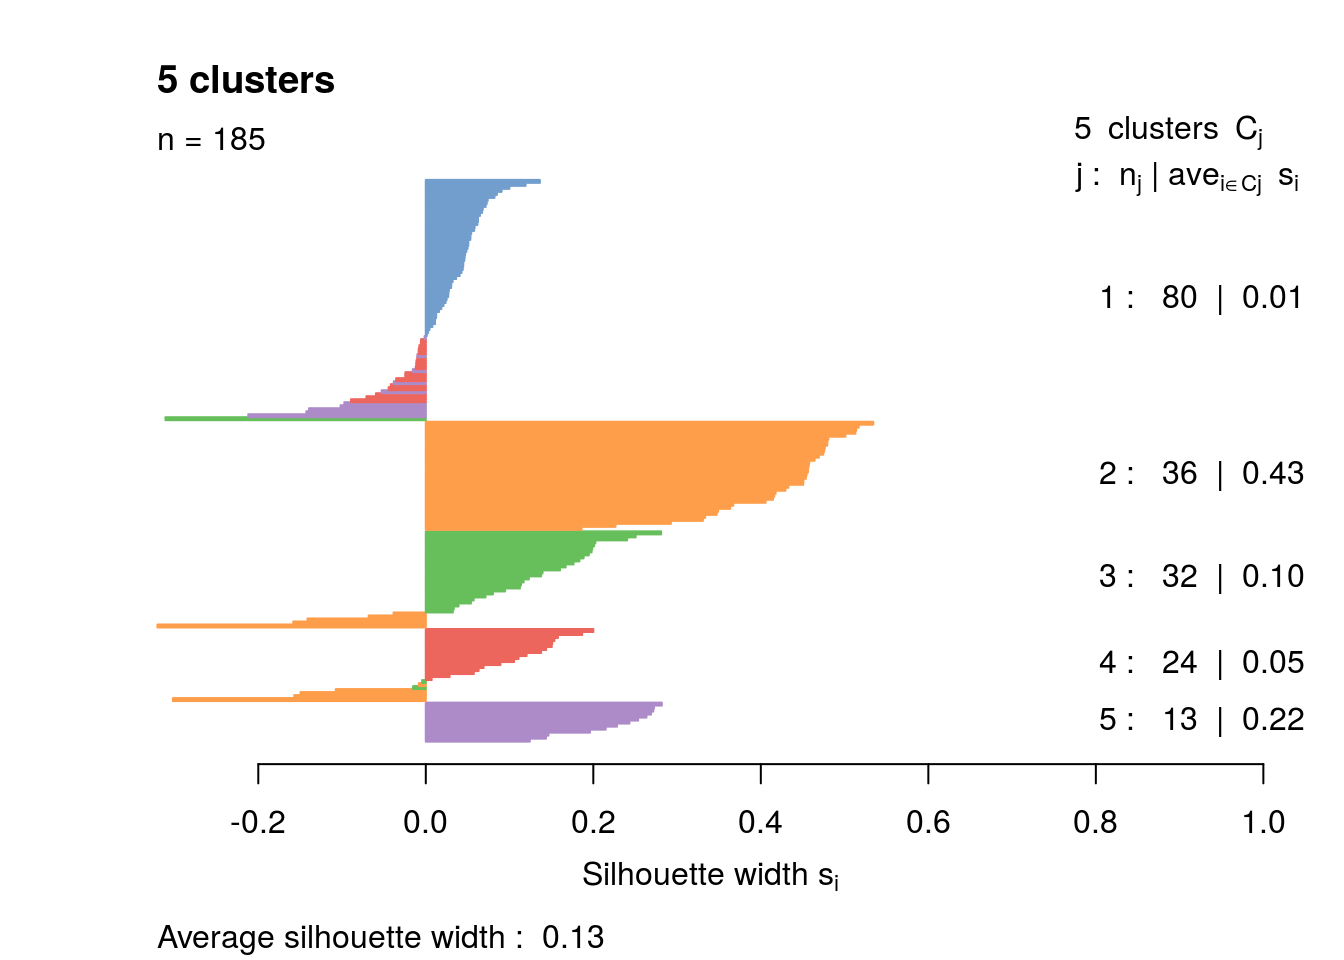
\includegraphics{0X.integrating-datasets_files/figure-latex/unnamed-chunk-13-1.pdf}

\hypertarget{limma-batch-correction}{%
\subsection{Limma Batch Correction}\label{limma-batch-correction}}

The \texttt{limma} package, a popular framework for the statistical analysis of RNA-seq, has a function \texttt{removeBatchEffect()} which will be used here to correct the normalized expression matrix \texttt{logcounts} across the two batches. The result will be assigned into the \texttt{assays} slot of the \texttt{sce} object as \texttt{limma\_corrected}, and then used for PCA, saving the result in the \texttt{reducedDim} slot as \texttt{"PCA\_limma"}.

\begin{Shaded}
\begin{Highlighting}[]
\NormalTok{limma_corrected <-}\StringTok{ }\NormalTok{limma}\OperatorTok{::}\KeywordTok{removeBatchEffect}\NormalTok{(}\KeywordTok{logcounts}\NormalTok{(sce), }\DataTypeTok{batch =}\NormalTok{ sce}\OperatorTok{$}\NormalTok{Sample)}
\KeywordTok{assay}\NormalTok{(sce, }\StringTok{"logcounts_limma"}\NormalTok{) <-}\StringTok{ }\NormalTok{limma_corrected }\CommentTok{## add new assay}

\NormalTok{pl <-}\StringTok{ }\KeywordTok{prcomp}\NormalTok{(}\KeywordTok{t}\NormalTok{(}\KeywordTok{assay}\NormalTok{(sce, }\StringTok{'logcounts_limma'}\NormalTok{)[hvg_genes, ]))}
\KeywordTok{reducedDim}\NormalTok{(sce, }\StringTok{"PCA_limma"}\NormalTok{) <-}\StringTok{ }\NormalTok{pl}\OperatorTok{$}\NormalTok{x[, }\DecValTok{1}\OperatorTok{:}\DecValTok{20}\NormalTok{]}
\end{Highlighting}
\end{Shaded}

\begin{Shaded}
\begin{Highlighting}[]
\KeywordTok{plotReducedDim}\NormalTok{(sce, }\DataTypeTok{use_dimred =} \StringTok{"PCA_limma"}\NormalTok{,}
               \DataTypeTok{colour_by=}\StringTok{"Sample"}\NormalTok{) }\OperatorTok{+}\StringTok{ }
\StringTok{    }\KeywordTok{ggtitle}\NormalTok{(}\StringTok{"PCA With limma removeBatchEffect() correction"}\NormalTok{)}
\end{Highlighting}
\end{Shaded}

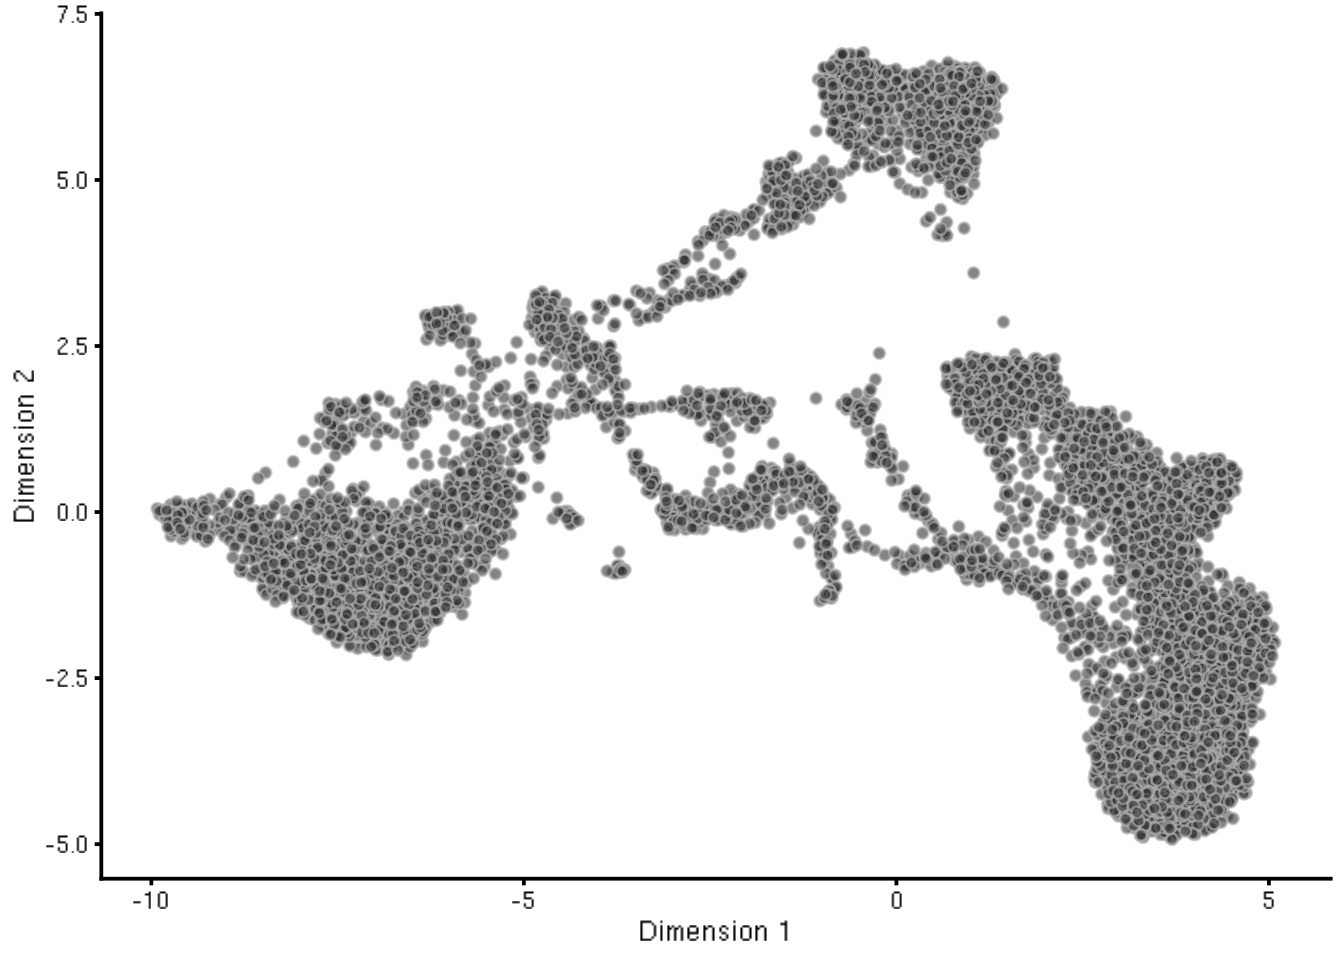
\includegraphics{0X.integrating-datasets_files/figure-latex/unnamed-chunk-15-1.pdf}

\hypertarget{mnn-approach}{%
\subsection{MNN Approach}\label{mnn-approach}}

The mutual nearest neighbors (MNN) approach within the \texttt{scran} package utilizes a novel approach to adjust for batch effects. The \texttt{fastMNN()} function returns a representation of the data with reduced dimensionality, which can be used in a similar fashion to other lower-dimensional representations such as PCA. In particular, this representation can be used for downstream methods such as clustering.

Where \texttt{fastMNN()} differs from other integration methods such as the limma approach above is that it does \emph{not} produce a batch-corrected expression matrix. Thus, the result from \texttt{fastMNN()} should solely be treated as a reduced dimensionality representation, suitable for direct plotting, TSNE/UMAP, clustering, and trajectory analysis that relies on such results. The already (batch) normalized (via \texttt{normalize()} and \texttt{multiBatchNorm()}) can be supplied to other statistical frameworks that are better suited to handle batch effects, such as in the case of differential expression.

\begin{Shaded}
\begin{Highlighting}[]
\CommentTok{## Basic method to run - not run}
\NormalTok{mnn_out <-}\StringTok{ }\KeywordTok{fastMNN}\NormalTok{(sce[hvg_genes, sce}\OperatorTok{$}\NormalTok{Sample }\OperatorTok{==}\StringTok{ "pbmc3k"}\NormalTok{],}
\NormalTok{                  sce[hvg_genes, sce}\OperatorTok{$}\NormalTok{Sample }\OperatorTok{==}\StringTok{ "pbmc4k"}\NormalTok{],}
                  \CommentTok{## subset.row = hvg_genes, ## same as subsetting above}
                  \DataTypeTok{k =} \DecValTok{20}\NormalTok{, }\DataTypeTok{d =} \DecValTok{50}\NormalTok{, }\DataTypeTok{approximate =} \OtherTok{TRUE}\NormalTok{,}
                  \DataTypeTok{BNPARAM =}\NormalTok{ BiocNeighbors}\OperatorTok{::}\KeywordTok{AnnoyParam}\NormalTok{(),}
                  \DataTypeTok{BPPARAM =}\NormalTok{ BiocParallel}\OperatorTok{::}\KeywordTok{multiCoreParam}\NormalTok{())}
\end{Highlighting}
\end{Shaded}

\begin{Shaded}
\begin{Highlighting}[]
\CommentTok{## Adding parallelization and Annoy method for approximate nearest neighbors}
\CommentTok{## this makes fastMNN significantly faster on large data}
\NormalTok{mnn_out <-}\StringTok{ }\KeywordTok{fastMNN}\NormalTok{(sce[hvg_genes, sce}\OperatorTok{$}\NormalTok{Sample }\OperatorTok{==}\StringTok{ "pbmc3k"}\NormalTok{],}
\NormalTok{                  sce[hvg_genes, sce}\OperatorTok{$}\NormalTok{Sample }\OperatorTok{==}\StringTok{ "pbmc4k"}\NormalTok{],}
                  \CommentTok{## subset.row = hvg_genes, ## same as subsetting above}
                  \DataTypeTok{k =} \DecValTok{20}\NormalTok{, }\DataTypeTok{d =} \DecValTok{50}\NormalTok{, }\DataTypeTok{approximate =} \OtherTok{TRUE}\NormalTok{,}
                  \DataTypeTok{BNPARAM =}\NormalTok{ BiocNeighbors}\OperatorTok{::}\KeywordTok{AnnoyParam}\NormalTok{(),}
                  \DataTypeTok{BPPARAM =}\NormalTok{ BiocParallel}\OperatorTok{::}\KeywordTok{MulticoreParam}\NormalTok{(}\DecValTok{8}\NormalTok{))}

\KeywordTok{reducedDim}\NormalTok{(sce, }\StringTok{"MNN"}\NormalTok{) <-}\StringTok{ }\NormalTok{mnn_out}\OperatorTok{$}\NormalTok{correct}
\end{Highlighting}
\end{Shaded}

\begin{Shaded}
\begin{Highlighting}[]
\KeywordTok{plotReducedDim}\NormalTok{(sce, }\DataTypeTok{use_dimred =} \StringTok{"MNN"}\NormalTok{,}
                    \DataTypeTok{colour_by=}\StringTok{"Sample"}\NormalTok{) }\OperatorTok{+}\StringTok{ }
\StringTok{    }\KeywordTok{ggtitle}\NormalTok{(}\StringTok{"MNN Ouput Reduced Dimensions"}\NormalTok{)}
\end{Highlighting}
\end{Shaded}

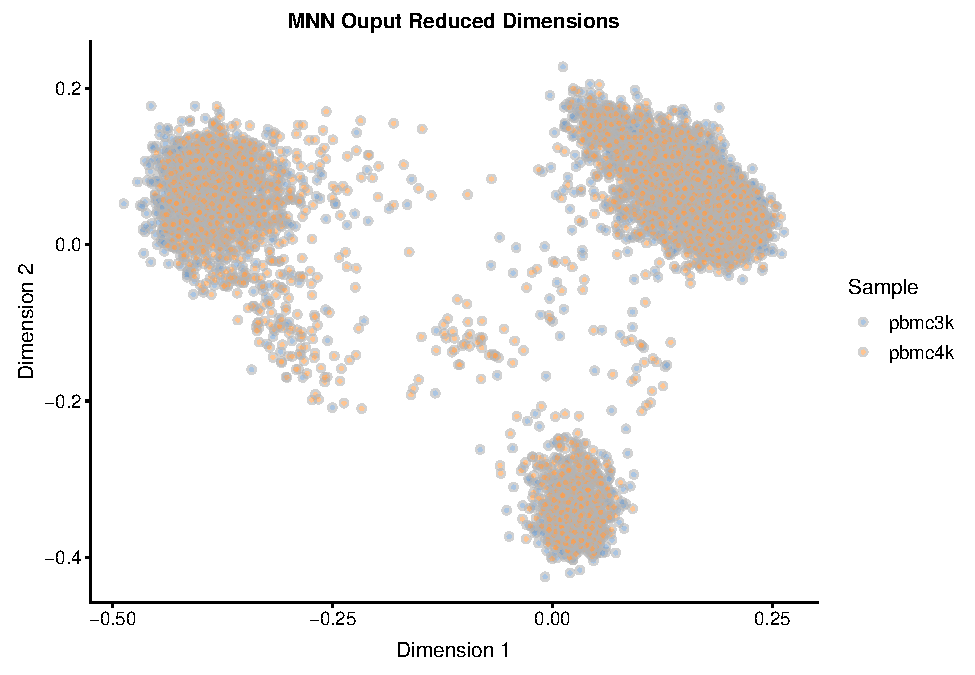
\includegraphics{0X.integrating-datasets_files/figure-latex/unnamed-chunk-18-1.pdf}

\hypertarget{session-info}{%
\section{Session Info}\label{session-info}}

\begin{Shaded}
\begin{Highlighting}[]
\KeywordTok{sessionInfo}\NormalTok{()}
\end{Highlighting}
\end{Shaded}

\begin{verbatim}
## R Under development (unstable) (2019-01-13 r75986)
## Platform: x86_64-apple-darwin18.2.0 (64-bit)
## Running under: macOS Mojave 10.14.3
## 
## Matrix products: default
## BLAS/LAPACK: /usr/local/Cellar/openblas/0.3.5/lib/libopenblasp-r0.3.5.dylib
## 
## locale:
## [1] en_US.UTF-8/en_US.UTF-8/en_US.UTF-8/C/en_US.UTF-8/en_US.UTF-8
## 
## attached base packages:
## [1] parallel  stats4    stats     graphics  grDevices utils     datasets 
## [8] methods   base     
## 
## other attached packages:
##  [1] BiocNeighbors_1.1.12        TENxPBMCData_1.1.0         
##  [3] HDF5Array_1.11.10           rhdf5_2.27.12              
##  [5] limma_3.39.12               scran_1.11.20              
##  [7] scater_1.11.12              ggplot2_3.1.0              
##  [9] SingleCellExperiment_1.5.2  SummarizedExperiment_1.13.0
## [11] DelayedArray_0.9.8          BiocParallel_1.17.17       
## [13] matrixStats_0.54.0          Biobase_2.43.1             
## [15] GenomicRanges_1.35.1        GenomeInfoDb_1.19.2        
## [17] IRanges_2.17.4              S4Vectors_0.21.10          
## [19] BiocGenerics_0.29.1        
## 
## loaded via a namespace (and not attached):
##  [1] bitops_1.0-6                  bit64_0.9-7                  
##  [3] httr_1.4.0                    dynamicTreeCut_1.63-1        
##  [5] tools_3.6.0                   R6_2.4.0                     
##  [7] irlba_2.3.3                   vipor_0.4.5                  
##  [9] DBI_1.0.0                     lazyeval_0.2.1               
## [11] colorspace_1.4-0              withr_2.1.2                  
## [13] tidyselect_0.2.5              gridExtra_2.3                
## [15] bit_1.1-14                    compiler_3.6.0               
## [17] labeling_0.3                  bookdown_0.9                 
## [19] scales_1.0.0                  stringr_1.4.0                
## [21] digest_0.6.18                 rmarkdown_1.11               
## [23] XVector_0.23.0                pkgconfig_2.0.2              
## [25] htmltools_0.3.6               rlang_0.3.1                  
## [27] RSQLite_2.1.1                 shiny_1.2.0                  
## [29] DelayedMatrixStats_1.5.2      dplyr_0.8.0.1                
## [31] RCurl_1.95-4.11               magrittr_1.5                 
## [33] BiocSingular_0.99.12          GenomeInfoDbData_1.2.0       
## [35] Matrix_1.2-15                 Rcpp_1.0.0                   
## [37] ggbeeswarm_0.6.0              munsell_0.5.0                
## [39] Rhdf5lib_1.5.1                viridis_0.5.1                
## [41] stringi_1.3.1                 yaml_2.2.0                   
## [43] edgeR_3.25.3                  zlibbioc_1.29.0              
## [45] plyr_1.8.4                    AnnotationHub_2.15.7         
## [47] grid_3.6.0                    blob_1.1.1                   
## [49] promises_1.0.1                ExperimentHub_1.9.1          
## [51] crayon_1.3.4                  lattice_0.20-38              
## [53] cowplot_0.9.4                 locfit_1.5-9.1               
## [55] knitr_1.21                    pillar_1.3.1                 
## [57] igraph_1.2.4                  glue_1.3.0                   
## [59] evaluate_0.13                 BiocManager_1.30.4           
## [61] httpuv_1.4.5.1                gtable_0.2.0                 
## [63] purrr_0.3.1                   assertthat_0.2.0             
## [65] xfun_0.5                      rsvd_1.0.0                   
## [67] mime_0.6                      xtable_1.8-3                 
## [69] later_0.8.0                   viridisLite_0.3.0            
## [71] tibble_2.0.1                  AnnotationDbi_1.45.0         
## [73] beeswarm_0.2.3                memoise_1.1.0                
## [75] statmod_1.4.30                interactiveDisplayBase_1.21.0
\end{verbatim}

\begin{Shaded}
\begin{Highlighting}[]
\KeywordTok{saveRDS}\NormalTok{(sce, }\StringTok{"_rfiles/_data/integration_sce.rds"}\NormalTok{, }\DataTypeTok{compress =} \StringTok{"xz"}\NormalTok{)}
\end{Highlighting}
\end{Shaded}

\hypertarget{workflow-clustering}{%
\chapter{Workflow: Clustering}\label{workflow-clustering}}

The purpose of this case study is to demonstrate various approaches to clustering scRNA-seq datasets using R/Bioconductor packages. In this workflow, we go from preprocessing the data to clustering the data. Furthermore, we highlight methods which are especially suitable for large datasets.

Here we will be working with a dataset from the \href{https://github.com/LuyiTian/CellBench_data}{CellBench} scRNA-seq benchmarking dataset collection. Specifically, we will be working with the \texttt{sc\_10x\_5cl} dataset, which contains 5 sorted cell lines that were sequencing on the 10X Genomics platform. We will use this to showcase our different clustering strategies.

\hypertarget{package-requirements-1}{%
\section{Package Requirements}\label{package-requirements-1}}

These packages will be required for working through the vignette, and can be installed by running the code below:

\begin{Shaded}
\begin{Highlighting}[]
\NormalTok{BiocManager}\OperatorTok{::}\KeywordTok{install}\NormalTok{(}\KeywordTok{c}\NormalTok{(}\StringTok{'scater'}\NormalTok{, }\StringTok{'scran'}\NormalTok{,}
                      \StringTok{'SC3'}\NormalTok{, }\StringTok{'clusterExperiment'}\NormalTok{, }\StringTok{'BiocNeighbors'}\NormalTok{,}
                      \StringTok{'BiocParallel'}\NormalTok{))}

\CommentTok{## suggested for combining plots}
\NormalTok{devtools}\OperatorTok{::}\KeywordTok{install_github}\NormalTok{(}\StringTok{'thomasp85/patchwork'}\NormalTok{)}
\end{Highlighting}
\end{Shaded}

\begin{Shaded}
\begin{Highlighting}[]
\KeywordTok{library}\NormalTok{(scater)}
\KeywordTok{library}\NormalTok{(scran)}
\KeywordTok{library}\NormalTok{(SC3)}
\KeywordTok{library}\NormalTok{(clusterExperiment)}
\KeywordTok{library}\NormalTok{(BiocNeighbors)}
\KeywordTok{library}\NormalTok{(BiocParallel)}
\KeywordTok{library}\NormalTok{(patchwork)}
\end{Highlighting}
\end{Shaded}

\hypertarget{loading-the-data-1}{%
\section{Loading the Data}\label{loading-the-data-1}}

To follow along with the workflow, we use the \href{https://github.com/LuyiTian/CellBench_data}{CellBench\_data} Github repository \texttt{data} folder's \texttt{sincell\_with\_class\_5cl.RData} workspace, which contains an object called \texttt{sc\_10x\_5cl\_qc}. While this data will eventually be submitted to ExperimentHub, a central repository for datasets, it is currently as yet unavailable there.

For the time being, the data can be found in this book's Github repo in the \texttt{\_rfiles/\_data} folder. The data arrives as a \texttt{SingleCellExperiment} class object.

\begin{Shaded}
\begin{Highlighting}[]
\NormalTok{sce <-}\StringTok{ }\KeywordTok{readRDS}\NormalTok{(}\StringTok{"_rfiles/_data/cellbench_sce_sc_10x_5cl_qc.rds"}\NormalTok{)}
\end{Highlighting}
\end{Shaded}

\hypertarget{understanding-the-data}{%
\section{Understanding the Data}\label{understanding-the-data}}

Within the cell metadata stored in the \texttt{colData} slot of our \texttt{sce} object, we see that information regarding the cell line of origin for each cell is stored under the column \texttt{cell\_line}, and furthermore can count the number of instances of each cell line present in the dataset as follows:

\begin{Shaded}
\begin{Highlighting}[]
\KeywordTok{table}\NormalTok{(sce}\OperatorTok{$}\NormalTok{cell_line)}
\end{Highlighting}
\end{Shaded}

\begin{verbatim}
## 
##   A549  H1975  H2228   H838 HCC827 
##   1244    515    751    840    568
\end{verbatim}

We will be using this information to illustrate our dimensionality reduction by highlighting each of the cell lines, and furthermore using this information to verify our clustering performance. While ground truth is not often known in practice, such benchmarking datasets are essential for validation of methods. While simulations are another source of establishing ground truth, this dataset is particularly appealing as it is derived under realistic experimental conditions.

\hypertarget{preprocessing-1}{%
\section{Preprocessing}\label{preprocessing-1}}

This dataset has already undergone cell quality control, so in this case we will skip this step (for this, we refer to the \protect\hyperlink{workflow-integrating-datasets}{Workflow on Integrating Datasets}. Thus, we will begin with the feature selection step and go on from there.

\hypertarget{feature-selection-1}{%
\section{Feature Selection}\label{feature-selection-1}}

In order to improve performance in terms of both speed and quality of results, we will start with defining a set of highly variable genes based on the biological coefficient of variability (see the \href{https://bioconductor.org/packages/devel/bioc/vignettes/scran/inst/doc/scran.html\#5_variance_modelling}{scran vignette} for details).

\begin{Shaded}
\begin{Highlighting}[]
\CommentTok{## Calculating highly variable genes -------------------}
\NormalTok{fit <-}\StringTok{ }\KeywordTok{trendVar}\NormalTok{(sce, }\DataTypeTok{parametric=}\OtherTok{TRUE}\NormalTok{, }\DataTypeTok{use.spikes =} \OtherTok{FALSE}\NormalTok{)}
\NormalTok{dec <-}\StringTok{ }\KeywordTok{decomposeVar}\NormalTok{(sce, fit)}
\NormalTok{hvg_genes <-}\StringTok{ }\KeywordTok{rownames}\NormalTok{(dec[dec}\OperatorTok{$}\NormalTok{FDR }\OperatorTok{<}\StringTok{ }\FloatTok{0.00001}\NormalTok{, ]) }\CommentTok{# 1874 genes}

\CommentTok{## remove uninteresting/unknown genes (ribosomal, mitochondrial)}
\NormalTok{bad_patterns <-}\StringTok{ 'RP[0-9]|^MT|[0-9][0-9][0-9][0-9]|^RPL|^RPS'}
\NormalTok{hvg_genes <-}\StringTok{ }\NormalTok{hvg_genes[}\OperatorTok{!}\KeywordTok{grepl}\NormalTok{(bad_patterns, hvg_genes)] }\CommentTok{# 1713 genes}

\CommentTok{## save the decomposed variance table and hvg_genes into metadata for safekeeping}
\KeywordTok{metadata}\NormalTok{(sce)}\OperatorTok{$}\NormalTok{hvg_genes <-}\StringTok{ }\NormalTok{hvg_genes}
\KeywordTok{metadata}\NormalTok{(sce)}\OperatorTok{$}\NormalTok{dec_var <-}\StringTok{ }\NormalTok{dec}
\end{Highlighting}
\end{Shaded}

\hypertarget{dimension-reduction}{%
\section{Dimension Reduction}\label{dimension-reduction}}

Here we will use PCA to calculate the first 20 principal components with our highly variable geneset, using the \texttt{irlba} method for a faster approximate version of the calculation. These PCs will then form the basis of our subsequent tSNE calculation.

\begin{Shaded}
\begin{Highlighting}[]
\NormalTok{sce <-}\StringTok{ }\KeywordTok{runPCA}\NormalTok{(sce, }\DataTypeTok{method =} \StringTok{"irlba"}\NormalTok{,}
             \DataTypeTok{ncomponents =} \DecValTok{20}\NormalTok{,}
             \DataTypeTok{feature_set =} \KeywordTok{metadata}\NormalTok{(sce)}\OperatorTok{$}\NormalTok{hvg_genes)}
\NormalTok{sce <-}\StringTok{ }\KeywordTok{runTSNE}\NormalTok{(sce,}
              \DataTypeTok{perplexity =} \DecValTok{30}\NormalTok{,}
              \DataTypeTok{feature_set =} \KeywordTok{metadata}\NormalTok{(sce)}\OperatorTok{$}\NormalTok{hvg_genes)}
\NormalTok{sce <-}\StringTok{ }\KeywordTok{runUMAP}\NormalTok{(sce,}
              \DataTypeTok{n_neighbors =} \DecValTok{15}\NormalTok{,}
              \DataTypeTok{feature_set =} \KeywordTok{metadata}\NormalTok{(sce)}\OperatorTok{$}\NormalTok{hvg_genes)}
\end{Highlighting}
\end{Shaded}

Here, we see that PCA nicely separates most of the cell lines, with the exception of HCC827 and H1975. On the other hand, tSNE nicely manages to separate the 5 cell lines, but interestingly produces two separate clusters for cell line H1975.

We leave it as an exercise to the interested reader to modify the essential tuning parameters, \texttt{perplexity}, and \texttt{n\_neighbors} for TSNE and UMAP respectively to see how the dimensionality reduction embeddings change. Here we have used the default parameters, but simply made them explicit. Information on these and other parameters can be seen by accessing the help for each function.

Note that clustering performance is \emph{not} necessarily dependent on the dimensionality reduction results (to answer this, it will depend on the specific clustering technique at hand).

However, clustering performance indeed \emph{may} be reflected in the dimensionality reduction results. For example, given the PCA result, we might expect some confusion between HCC827 and H1975, and based on the UMAP results, we might possibly even see two clusters within the H1975 cell line. Note however that these dimensionality reduction embeddings are also a function of the tuning parameters noted above.

\begin{Shaded}
\begin{Highlighting}[]
\NormalTok{gPCA <-}\StringTok{ }\KeywordTok{plotReducedDim}\NormalTok{(sce, }\StringTok{"PCA"}\NormalTok{, }\DataTypeTok{colour_by =} \StringTok{"cell_line"}\NormalTok{)}
\NormalTok{gTSNE <-}\StringTok{ }\KeywordTok{plotReducedDim}\NormalTok{(sce, }\StringTok{"TSNE"}\NormalTok{, }\DataTypeTok{colour_by =} \StringTok{"cell_line"}\NormalTok{)}
\NormalTok{gUMAP <-}\StringTok{ }\KeywordTok{plotReducedDim}\NormalTok{(sce, }\StringTok{"UMAP"}\NormalTok{, }\DataTypeTok{colour_by =} \StringTok{"cell_line"}\NormalTok{)}
\NormalTok{patchwork}\OperatorTok{::}\KeywordTok{wrap_plots}\NormalTok{(gPCA, gTSNE, gUMAP, }\DataTypeTok{heights =} \DecValTok{1}\NormalTok{, }\DataTypeTok{widths =} \DecValTok{1}\NormalTok{, }\DataTypeTok{ncol =} \DecValTok{3}\NormalTok{)}
\end{Highlighting}
\end{Shaded}

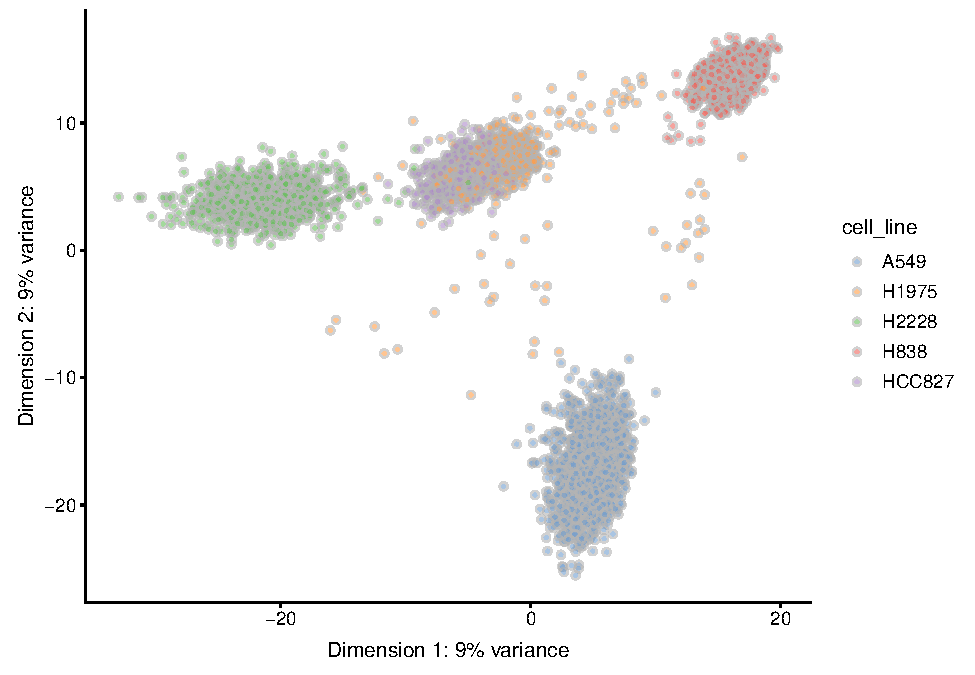
\includegraphics{0Y.clustering-datasets_files/figure-latex/unnamed-chunk-8-1.pdf}

\hypertarget{clustering}{%
\section{Clustering}\label{clustering}}

Here we highlight different frameworks for clustering. The first two, using the \texttt{sc3} and \texttt{clusterExperiment} Bioconductor packages, are fuller implementations that can test across multiple parametrizations and furthermore inspect the quality of the clustering results. The \texttt{BiocNeighbors} package is briefly highlighted to show a minimal alternative to clustering that emphasizes speed.

\hypertarget{sc3}{%
\subsection{SC3}\label{sc3}}

The \texttt{sc3} package provides a simple framework that allows users to test for many k's, e.g.~numbers of clusters, and subsequently compare the results from these differing k's in both quantitative and qualitative ways to pick an optimal k result. Below, we first set an essential \texttt{rowData} feature required by the package to run. Subsequently, we run the \texttt{sc3()} function in this example using a subset of the data (only the highly variable genes, \texttt{hvg\_genes}, testing k's 3 through 6.

\begin{Shaded}
\begin{Highlighting}[]
\CommentTok{## SC3 requires this column to be appended}
\KeywordTok{rowData}\NormalTok{(sce)}\OperatorTok{$}\NormalTok{feature_symbol <-}\StringTok{ }\KeywordTok{rownames}\NormalTok{(sce) }

\CommentTok{## SC3 will return an SCE object with appended "sc3_" columns}
\NormalTok{sce <-}\StringTok{ }\KeywordTok{sc3}\NormalTok{(sce[}\KeywordTok{metadata}\NormalTok{(sce)}\OperatorTok{$}\NormalTok{hvg_genes, ],}
          \DataTypeTok{ks =} \DecValTok{3}\OperatorTok{:}\DecValTok{6}\NormalTok{,}
          \DataTypeTok{k_estimator =} \OtherTok{TRUE}\NormalTok{)}
\end{Highlighting}
\end{Shaded}

After using \texttt{sc3()}, the function returns the original \texttt{SingleCellExperiment} object, but with new columns in \texttt{colData(sce)} corresponding to the different \texttt{ks} supplied to the function, as well as a full representation of the analysis that is stored in \texttt{metadata(sce)\$sc3}, which includes an estimate of the optimal \texttt{k} (as dictated by the \texttt{k\_estimator\ =\ TRUE} argument above).

Below, we show the clustering results of the \texttt{ks} we supplied, 3 through 6, shown on the TSNE representation of the data. We use the \texttt{scater} package function \texttt{plotReducedDim()} to produce the individual plots, and for the sake of this vignette, wrap them together into a single plot using the \texttt{patchwork} package.

\begin{Shaded}
\begin{Highlighting}[]
\CommentTok{## Basic code:}
\NormalTok{g3 <-}\StringTok{ }\KeywordTok{plotReducedDim}\NormalTok{(sce, }\DataTypeTok{use_dimred =} \StringTok{"TSNE"}\NormalTok{, }\DataTypeTok{colour_by =} \StringTok{"sc3_3_clusters"}\NormalTok{)}
\NormalTok{g4 <-}\StringTok{ }\KeywordTok{plotReducedDim}\NormalTok{(sce, }\DataTypeTok{use_dimred =} \StringTok{"TSNE"}\NormalTok{, }\DataTypeTok{colour_by =} \StringTok{"sc3_4_clusters"}\NormalTok{)}
\NormalTok{g5 <-}\StringTok{ }\KeywordTok{plotReducedDim}\NormalTok{(sce, }\DataTypeTok{use_dimred =} \StringTok{"TSNE"}\NormalTok{, }\DataTypeTok{colour_by =} \StringTok{"sc3_5_clusters"}\NormalTok{)}
\NormalTok{g6 <-}\StringTok{ }\KeywordTok{plotReducedDim}\NormalTok{(sce, }\DataTypeTok{use_dimred =} \StringTok{"TSNE"}\NormalTok{, }\DataTypeTok{colour_by =} \StringTok{"sc3_6_clusters"}\NormalTok{)}
\NormalTok{patchwork}\OperatorTok{::}\KeywordTok{wrap_plots}\NormalTok{(g3, g4, g5, g6, }\DataTypeTok{widths =} \DecValTok{1}\NormalTok{, }\DataTypeTok{heights =} \DecValTok{1}\NormalTok{, }\DataTypeTok{ncol =} \DecValTok{1}\NormalTok{)}
\end{Highlighting}
\end{Shaded}

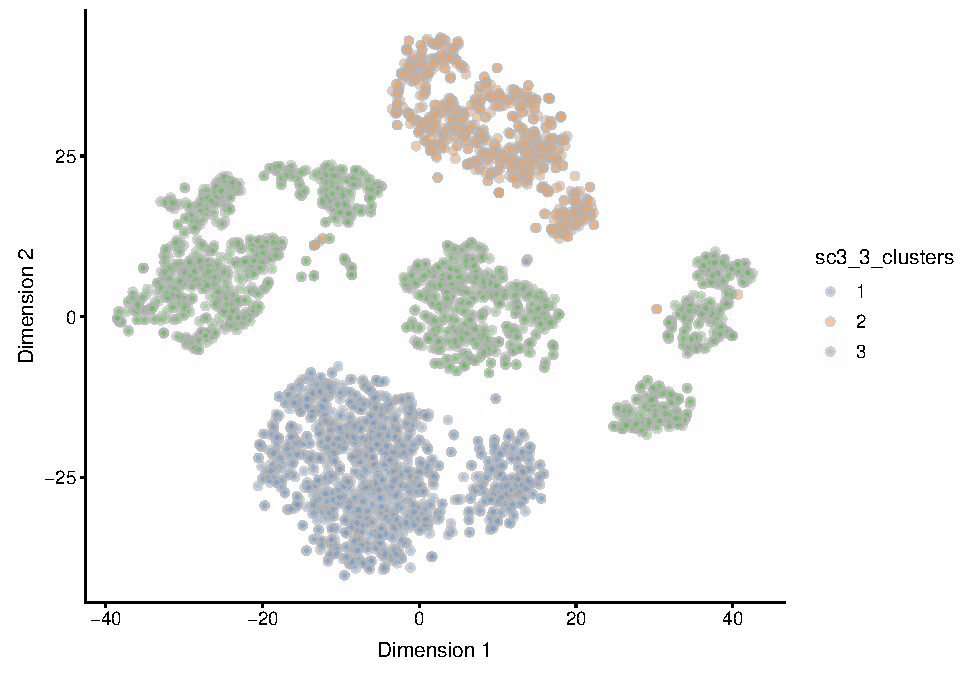
\includegraphics{0Y.clustering-datasets_files/figure-latex/unnamed-chunk-10-1.pdf}

The \texttt{sc3} package contains many more utilities for exploring the stability of clustering and can even produce differential expression analysis results using the \texttt{biology\ =\ TRUE} argument within the \texttt{sc3()} function. We leave it to the interested reader to \href{https://bioconductor.org/packages/release/bioc/html/SC3.html}{learn more about \texttt{sc3}} via their vignette.

\hypertarget{clusterexperiment}{%
\subsection{clusterExperiment}\label{clusterexperiment}}

The \texttt{clusterExperiment} package uses the function \texttt{RSEC()} to calculate clusters across various parametrizations, and contains multiple parameters to do so. Here, we specify the parametrizations to iterate over using the \texttt{alphas} and \texttt{k0s} arguments below. We refer the reader to the help page for \texttt{?RSEC} to learn more about the different parameters. In the end, this exhaustive exercise is used to ultimately determine a consensus clustering that combines the information learned from the various parametrizations.

\begin{Shaded}
\begin{Highlighting}[]
\NormalTok{rsec <-}\StringTok{ }\KeywordTok{RSEC}\NormalTok{(sce[}\KeywordTok{metadata}\NormalTok{(sce)}\OperatorTok{$}\NormalTok{hvg_genes, ],}
            \DataTypeTok{reduceMethod =} \StringTok{"PCA"}\NormalTok{,}
            \DataTypeTok{nReducedDims =} \DecValTok{20}\NormalTok{,}
            \DataTypeTok{alphas =} \KeywordTok{c}\NormalTok{(}\FloatTok{0.1}\NormalTok{, }\FloatTok{0.3}\NormalTok{), }\DataTypeTok{k0s =} \DecValTok{4}\OperatorTok{:}\DecValTok{6}\NormalTok{,}
            \DataTypeTok{consensusMinSize =} \DecValTok{50}\NormalTok{)}

\KeywordTok{metadata}\NormalTok{(sce)}\OperatorTok{$}\NormalTok{rsec <-}\StringTok{ }\NormalTok{rsec}
\KeywordTok{colData}\NormalTok{(sce)}\OperatorTok{$}\NormalTok{rsec_consensus_clusters <-}\StringTok{ }\KeywordTok{as.factor}\NormalTok{(}\KeywordTok{clusterMatrix}\NormalTok{(rsec)}\OperatorTok{$}\NormalTok{mergeClusters)}
\end{Highlighting}
\end{Shaded}

Once again, we refer the interested reader to the \href{https://bioconductor.org/packages/release/bioc/html/clusterExperiment.html}{vignette for \texttt{clusterExperiment}} to learn more about extended functionality for visualizing the data and about the specifics of the clustering workflow.

\hypertarget{biocneighbors}{%
\subsection{BiocNeighbors}\label{biocneighbors}}

The \texttt{BiocNeighbors} package provides a lower-level method for clustering of data. Under the hood, it provides various types of clustering algorithms, as specified through the \texttt{BNPARAM} class object. This \texttt{BNPARAM} object can be passed into the \texttt{BiocNeighbors} clustering function, \texttt{findKNN()}, as well as other functions that support \texttt{BNPARAM}.

The \texttt{BiocNeighbors} packaged is especially designed for developers to enable a unified interface for clustering algorithm specification, allowing for the separation of clustering functionality from the main function.

\bibliography{book.bib,packages.bib}


\end{document}
